
%===================================== CHAP 7 =================================

The results of this work are presented in two sections. The first section is the results of the sample preparation including polishing, oven annealing, lithography and contact deposition, and of the samples. The second section contains results from the study of fiber cores including of electrical measurements, SEM imaging and EDS. Further results from X-ray diffraction and Electron-probe micro-analysis of the same fibers are presented to discuss how the fiber core crystal structure and composition are influenced by fiber drawing and laser annealing.

\section{Fiber Polishing}
The polishing techniques were successful in preparing longitudinal cross sections of fibres cores for measurement. Very small amounts of tilt were observed during polishing leading to one end of the fiber core being exposed first. This was insignificant in practice as $ > 1 \si{\cm}$ lengths of fiber core with a diameter of $50 \si{\micro\meter}$ could be polished to expose the core across the entire length. Fibers with core sizes down to $7 \si{\micro\meter}$ were prepared with these methods. Using $9 \si{\micro\meter}$ diamond solution on a Struers MD Plan cloth gave the best results but had a very low polishing rate. Alternatively, in order to cut out excessive waste of diamond abrasive, the hand polishing jig was used on $15$ and $10 \si{\micro\meter}$ SiC paper to remove the majority of the cladding, then the sample was swithched to the Tegramin polished with $9 \si{\micro\meter}$ diamond solution to expose the core. This method produced some chipping of the fiber edges but the core was not affected. The surface roughness achieved with machine polishing is shown in figure \ref{surface_roughness}. If necessary oxide polishing with $0.1 \si{\micro\meter}$ alumina suspension or vibrational polishing with a Buehler Vibromet could improve on these results.


\begin{figure}[h]
  \centering
  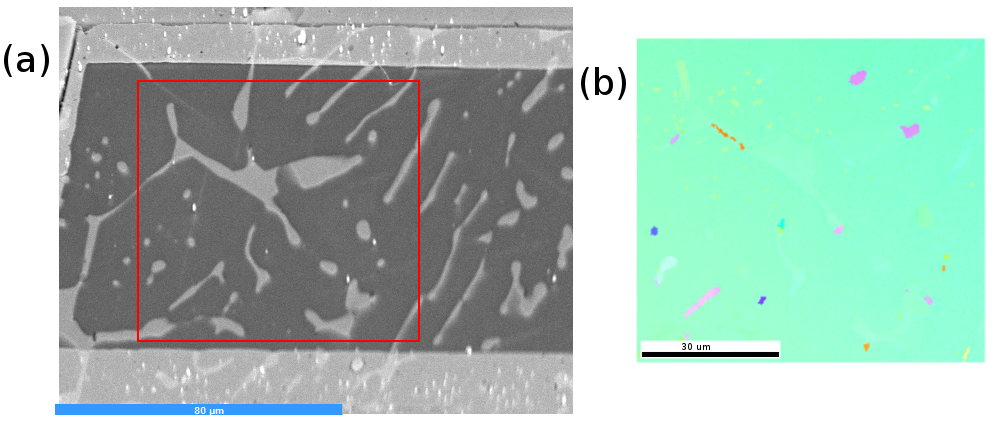
\includegraphics[width=\textwidth]{fig/ebsd_machinepolish.png}
  \caption{EBSD results of GaSb fiber after polish to $1\si{\micro\meter}$ \cite{Song2019LaserFibres}. A large improvement is seen over the hand polished fiber results in figure \ref{fig:ebsd} where scratches obscured the crystal orientation of some areas. }
  \label{fig:ebsd_2}
\end{figure}% %blank line makes figures vertical


\begin{figure}[h]
    \centering
    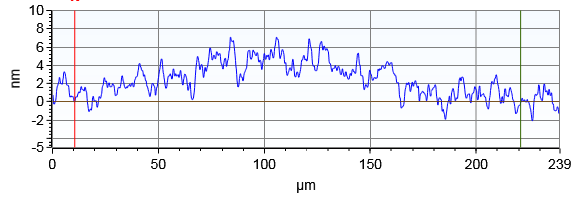
\includegraphics[width=\textwidth]{fig/Results/polished2.png}
    \caption{Surface roughness of a polished fiber core}
    \label{surface_roughness}
\end{figure}

\begin{figure}[h]
    \centering
    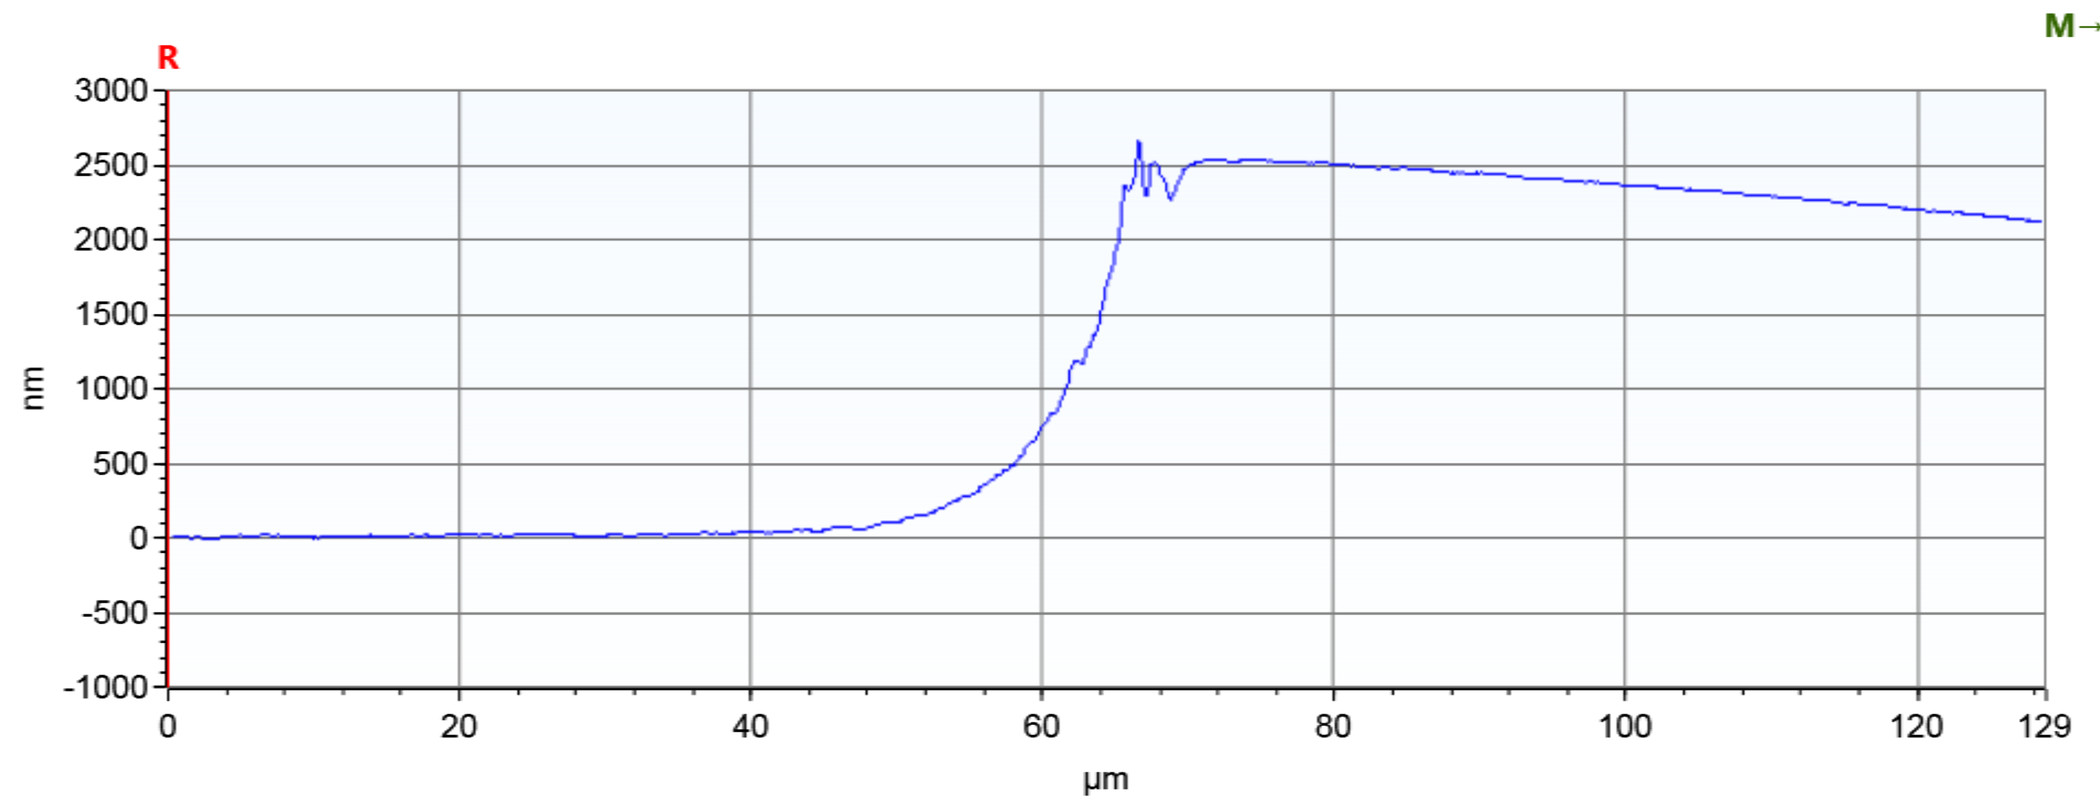
\includegraphics[width=\textwidth]{fig/Results/900expoydge2-1.jpg}    \caption{Profile plot showing relief between the cladding of a polished fiber sample and the epoxy}
    \label{profile}
\end{figure}

\subsection{Stress and Cracking}

Polishing of fibers inevitably led to cracking of the cladding and core regardless of the polishing method used. It is well documented that the as-drawn fibers contain stress, but it remains an open question in the group whether the cracking observed during polishing results solely from internal stress, or may also be caused by forces experienced during the polishing procedure \cite{Healy2018AFibres, Fokine2017LaserFibers, LapointeElectricalFibres, KristinKristin_thesis_final}. 

A typical pattern of cracking is shown in figure 1a. A long parallel crack is seen running parrallel to the fiber core, and transverse cracks cut across the core and continue propagating into the cladding. It was observed that cracks would form before the core was entirely exposed as seen in figure 1b, indicating that these were not due to polishing forces.  This does not eliminate the possibility of a bending force originating from shrinkage during the curing of the epoxy. The appearance of some long sections of crack-free core suggest this is unlikely as these forces should be similar across samples. It is tempting to try to link to fracture patterns to the Si crystal planes due to the remarkable symmetry seen \cite{KristinKristin_thesis_final}, however the appearance across fibers that are not known to be single crystalline suggests geometry may play a more important factor. 

Examples of annealed fibers can be seen in figures 4.4. The annealing experiments were not performed in a rigorous way. They were done to see if major improvements could be seen, and thus only some qualitative remarks can be made (see \cite{Zhao2018EffectsFiber} for a similar study). Annealed fibers showed large crack-free regions, but these were also accompanied by more extreme cracking of the glass. Cracking appears to be the mechanism for release rather than a relaxation through the softening of the glass during oven annealing. Diffusion of the coating material into the cladding during fiber drawing may have changed the properties of the glass near the fiber core and may be a cause of this tendency for greater cracking after oven annealing. While these results are not conclusive, a follow up is suggested including raman analysis to quantify the results. 



 
\begin{figure}[h]
 %h here H requires float, exactly here, h! overide latex
\centering
\begin{subfigure}{\textwidth}
  \centering
  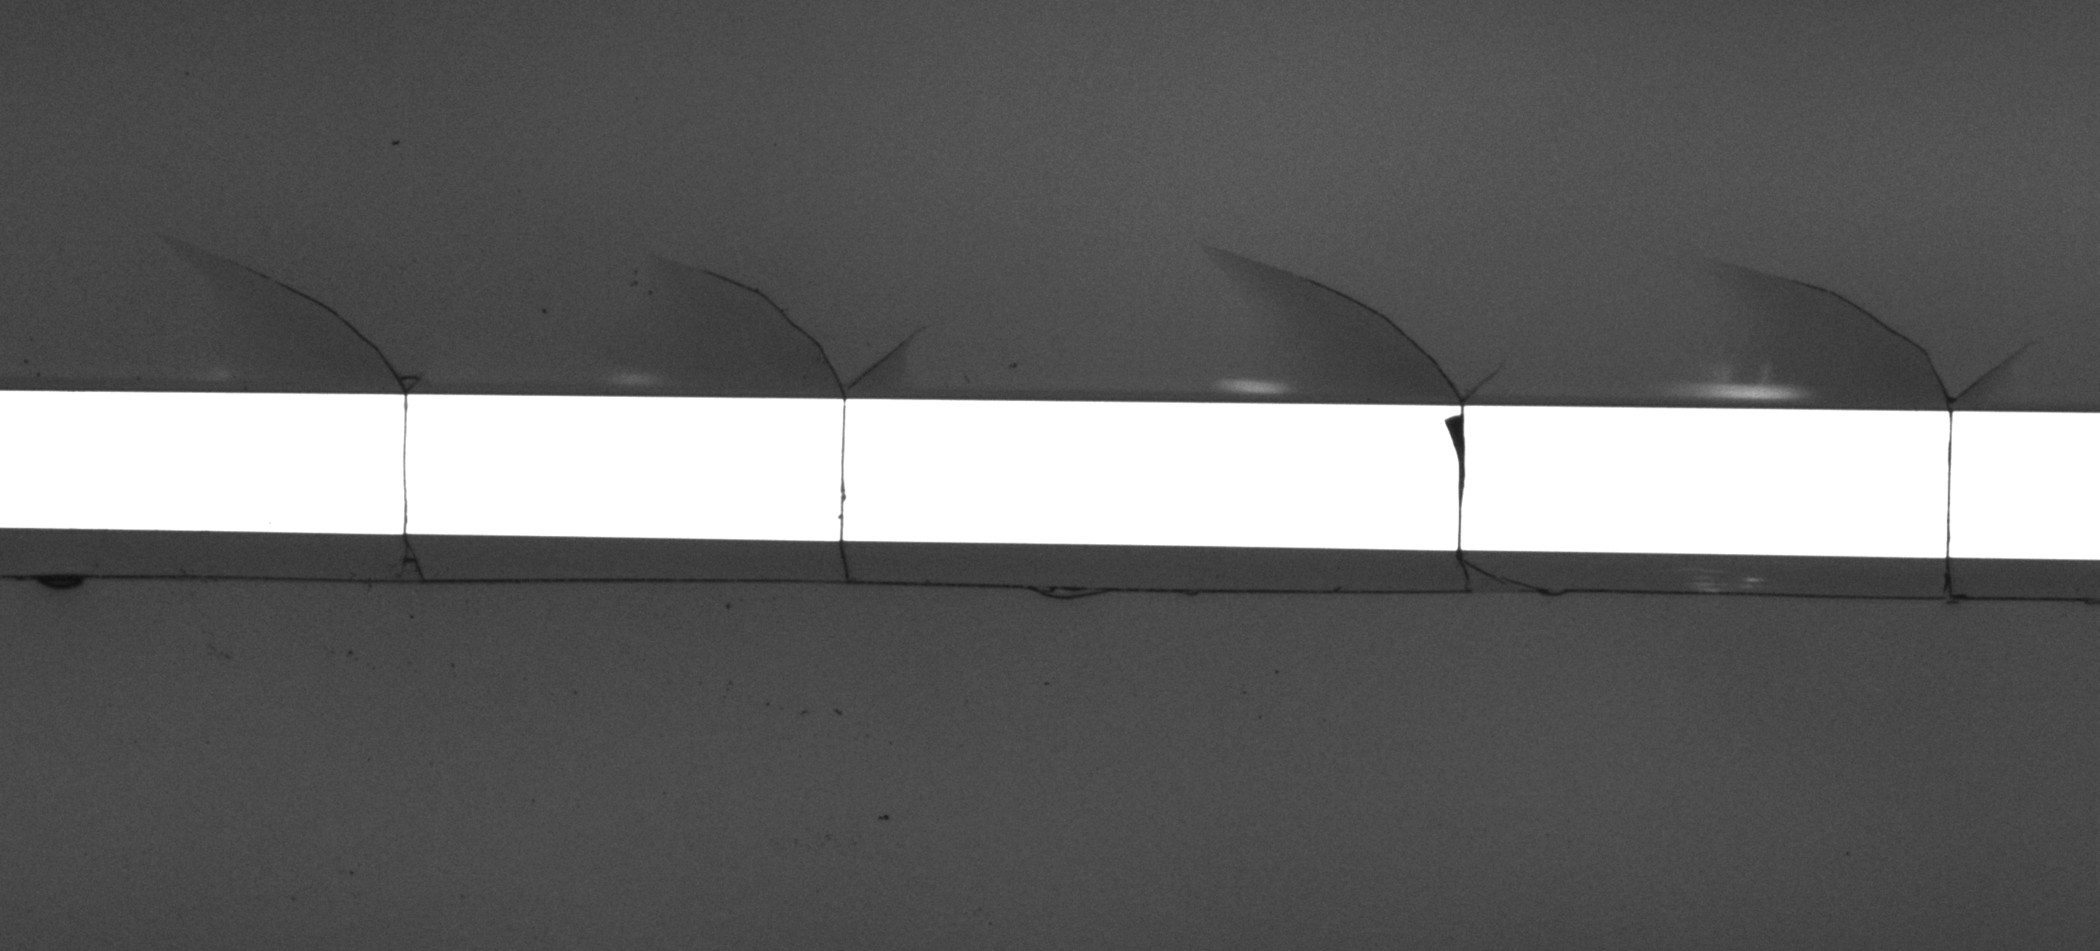
\includegraphics[width=\linewidth]{fig/polishing/Siedit.jpg}
  %\caption{1a}
  
\end{subfigure}% %blank line makes figures vertical

\begin{subfigure}{\textwidth}
  \centering
  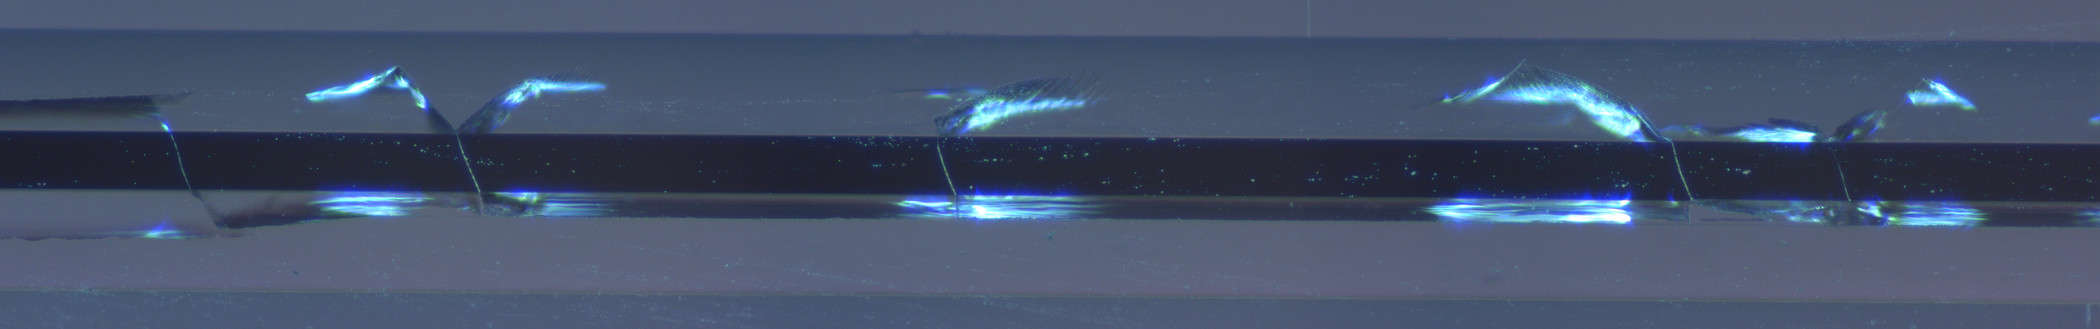
\includegraphics[width=\linewidth]{fig/polishing/e944.jpg}
  %\caption{1a}
  
\end{subfigure}% %blank line makes figures vertical
\caption{Si A ($55 \si{\micro\meter}$ core) and Si B ($65 \si{\micro\meter}$ core)fibers showing similar cracking features. }
\end{figure}

\begin{figure}
\begin{subfigure}{\textwidth}
  \centering
  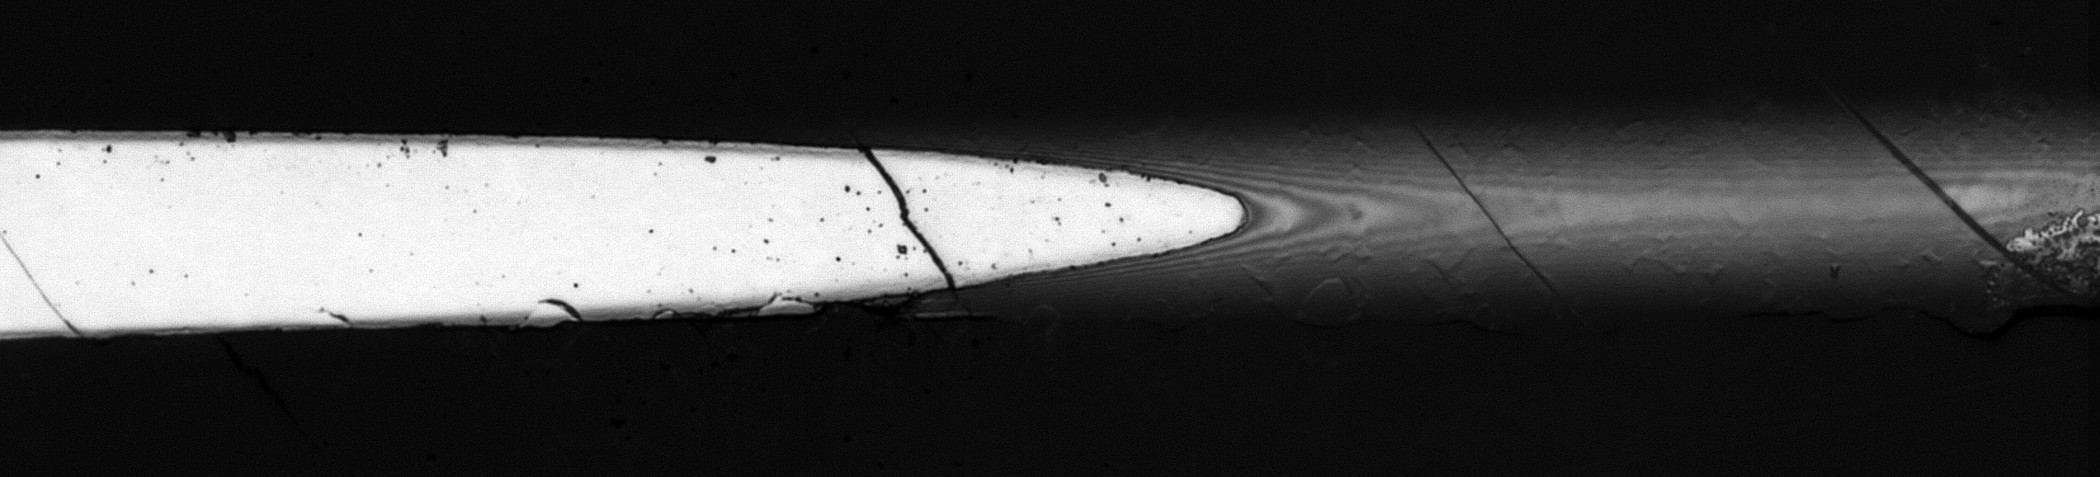
\includegraphics[width=\linewidth]{fig/polishing/SiGe_edit.jpg}
  %\caption{1a}\label{fig:sfig2}
\end{subfigure}% %blank line makes figures vertical

\begin{subfigure}{\textwidth}
  \centering
  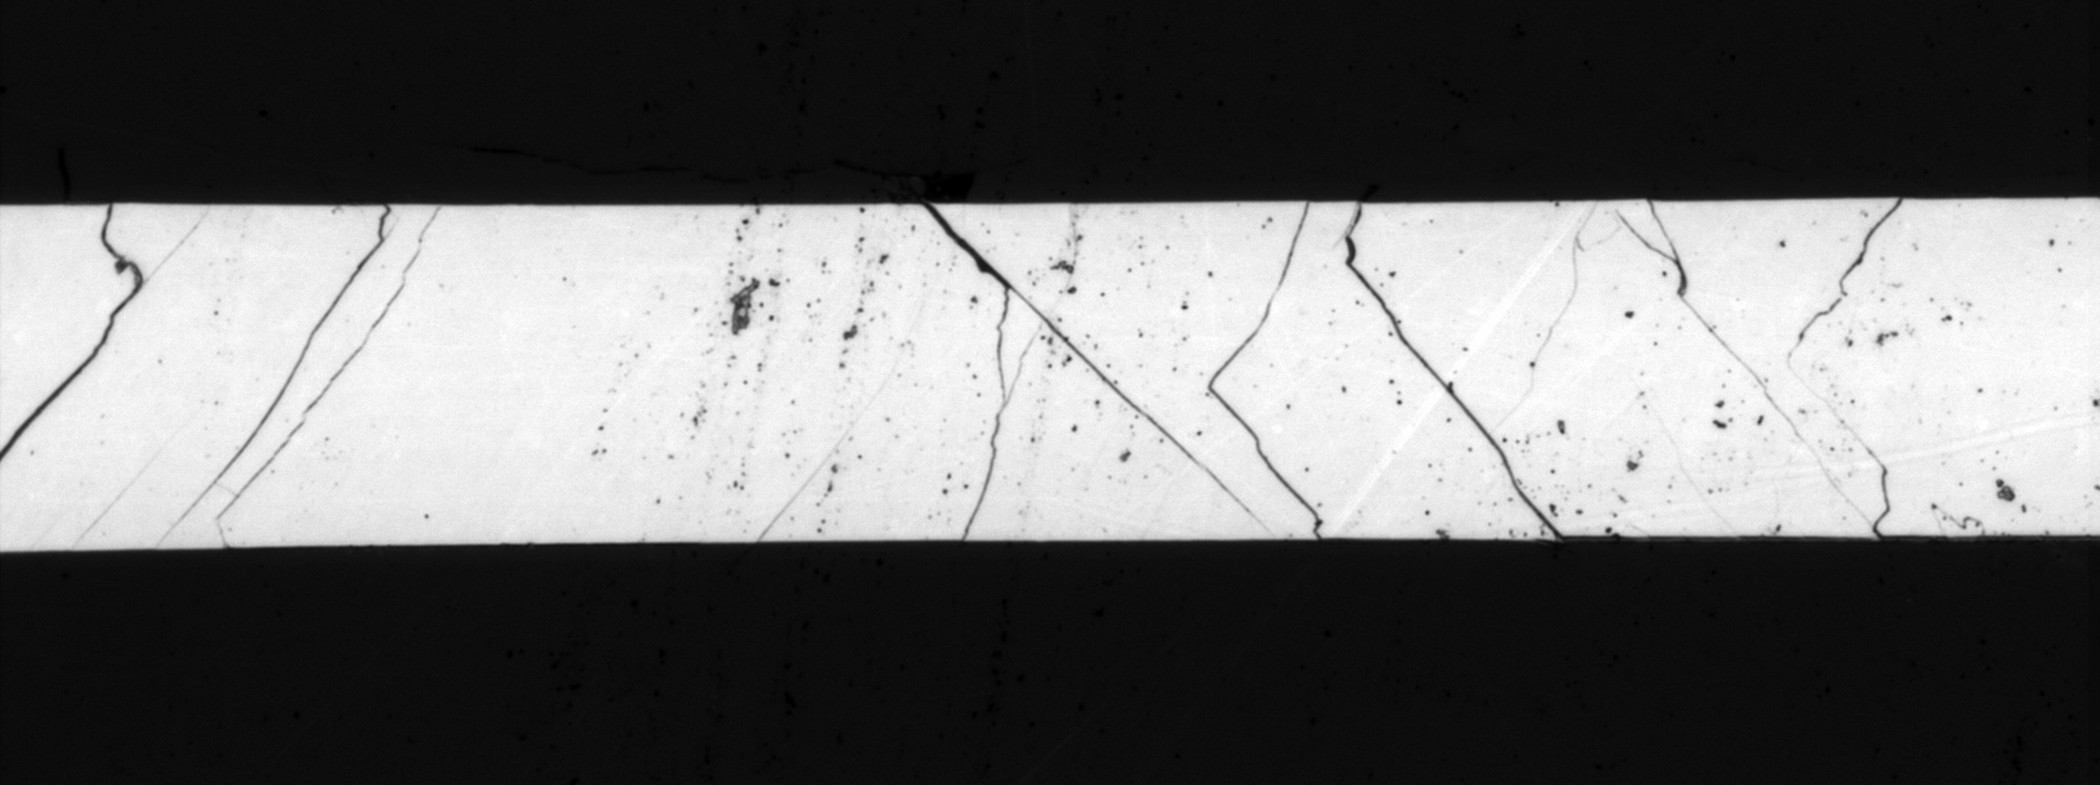
\includegraphics[width=\linewidth]{fig/polishing/SiGe2_edit.jpg}
  %\caption{1b}
 
\end{subfigure}
\caption{Larger core SiGe fibers showed larger stresses and heavy cracking.}
\label{fig:si_sige}
\end{figure}


%\begin{figure}[h]
 %h here H requires float, exactly here, h! overide latex
%\centering
%\begin{subfigure}{.7\textwidth}
%  \centering
%  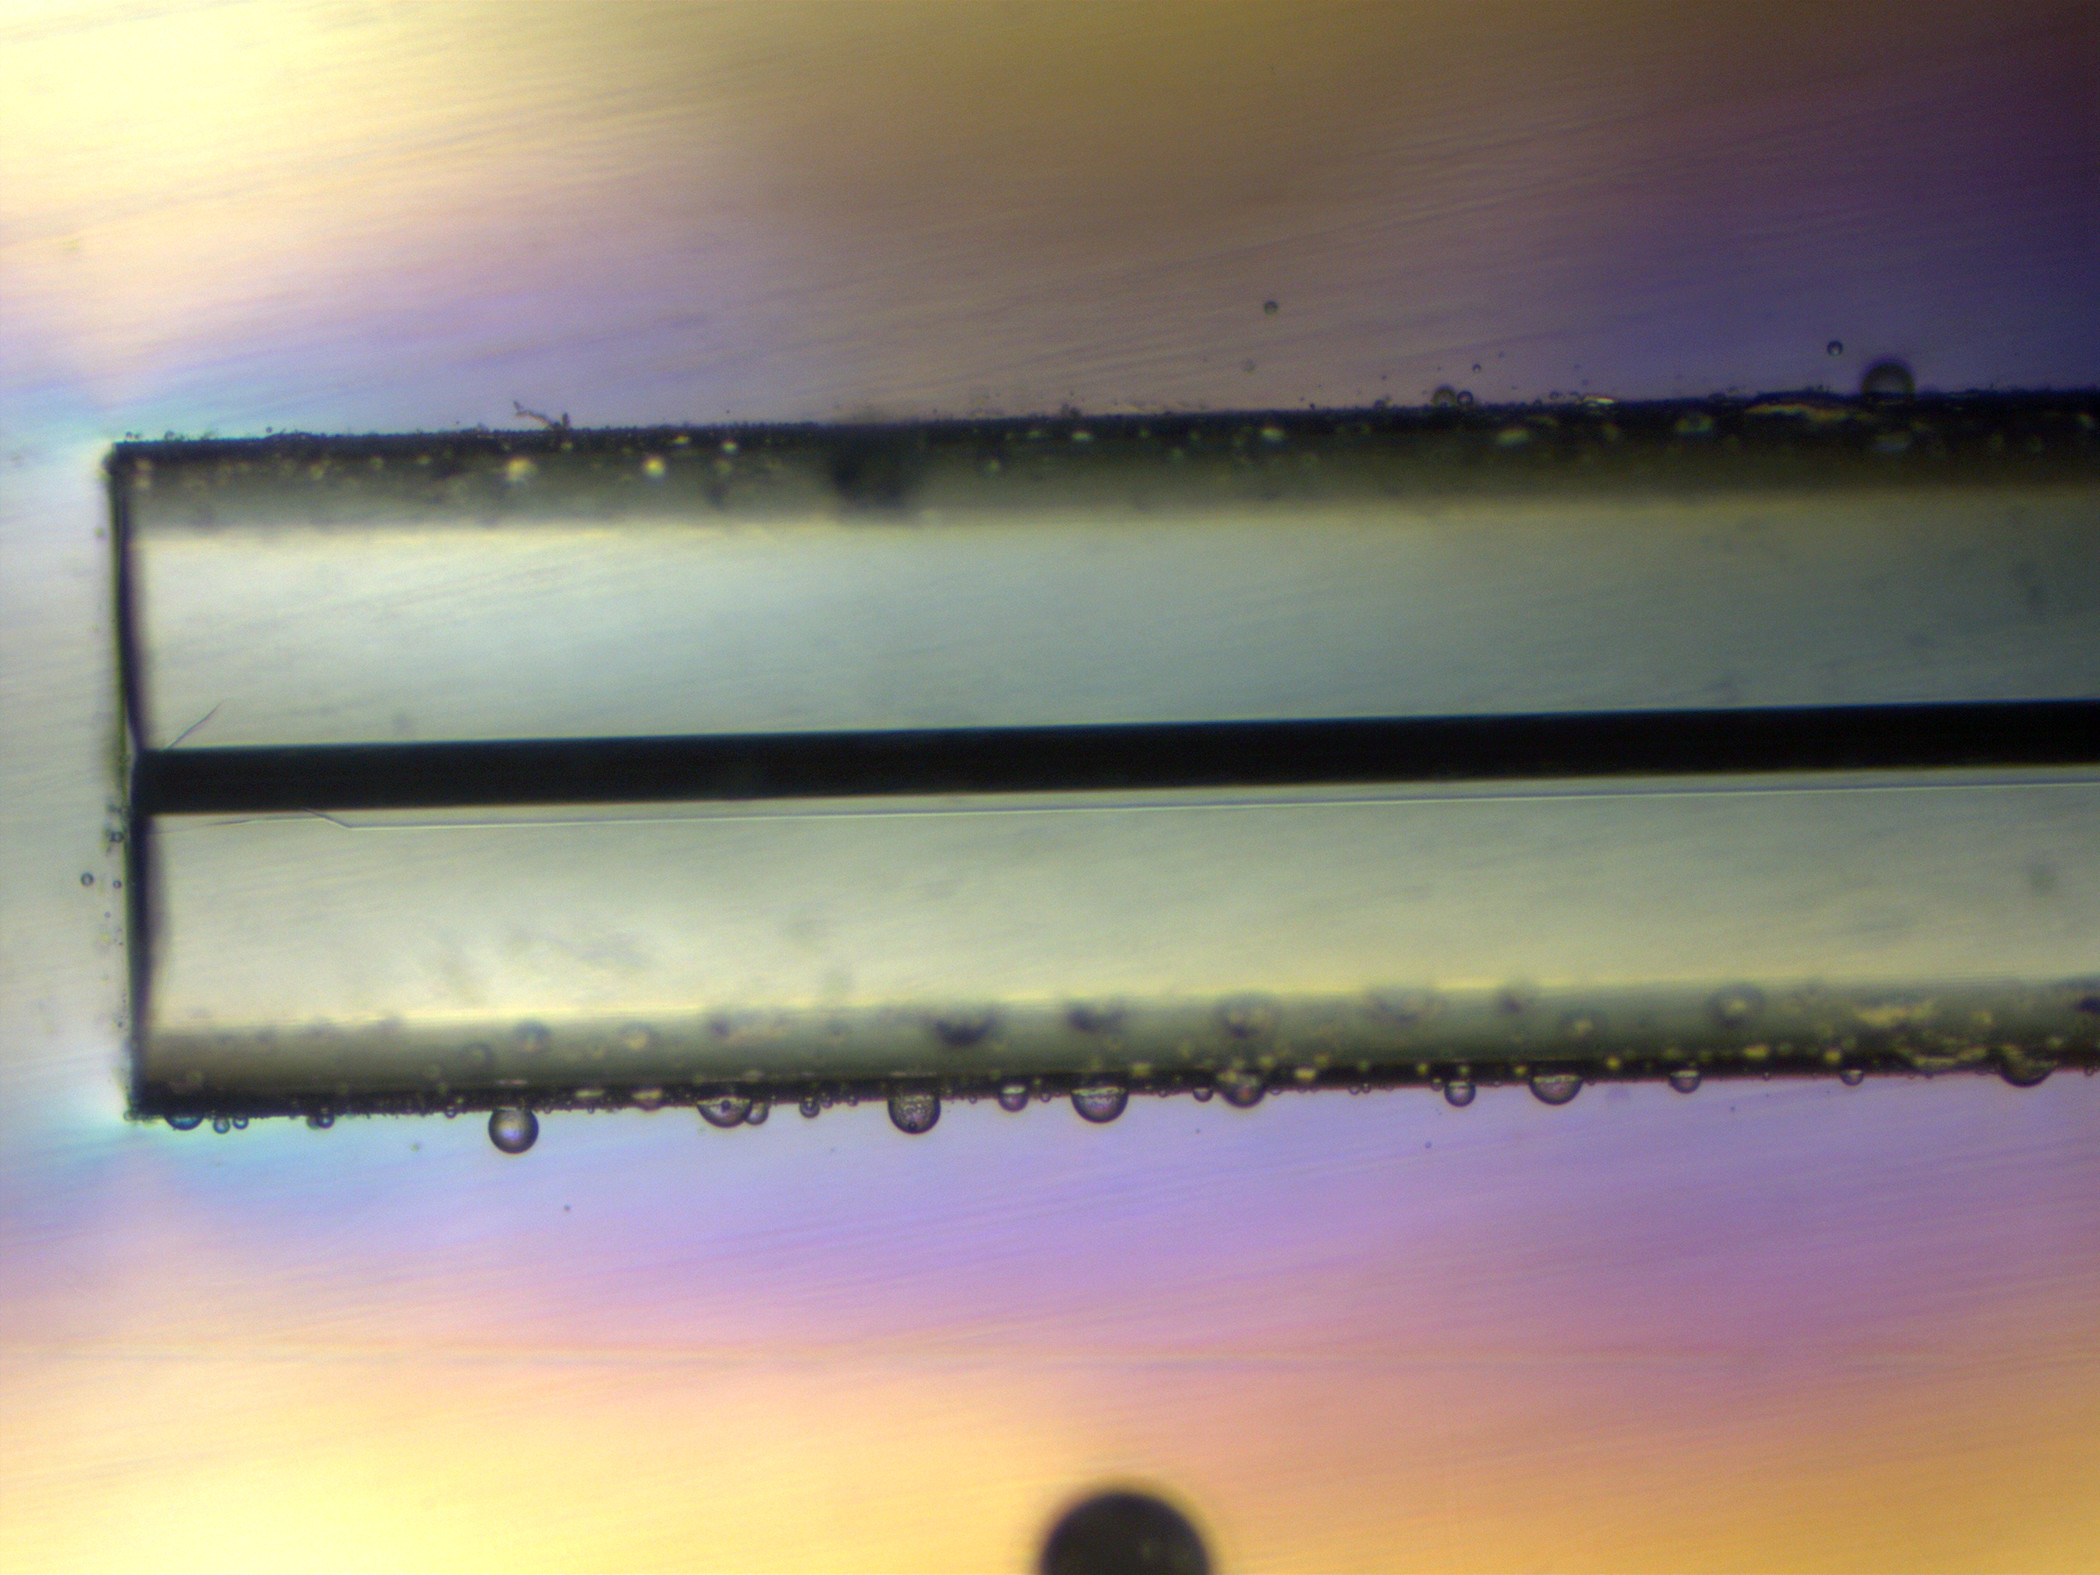
\includegraphics[width=\linewidth]{fig/polishing/parallelcrack.jpg}
  %\caption{1a}
%  \label{fig:sfig1}
%\end{subfigure}% %blank line makes figures vertical

%\begin{subfigure}{.7\textwidth}
%  \centering
%  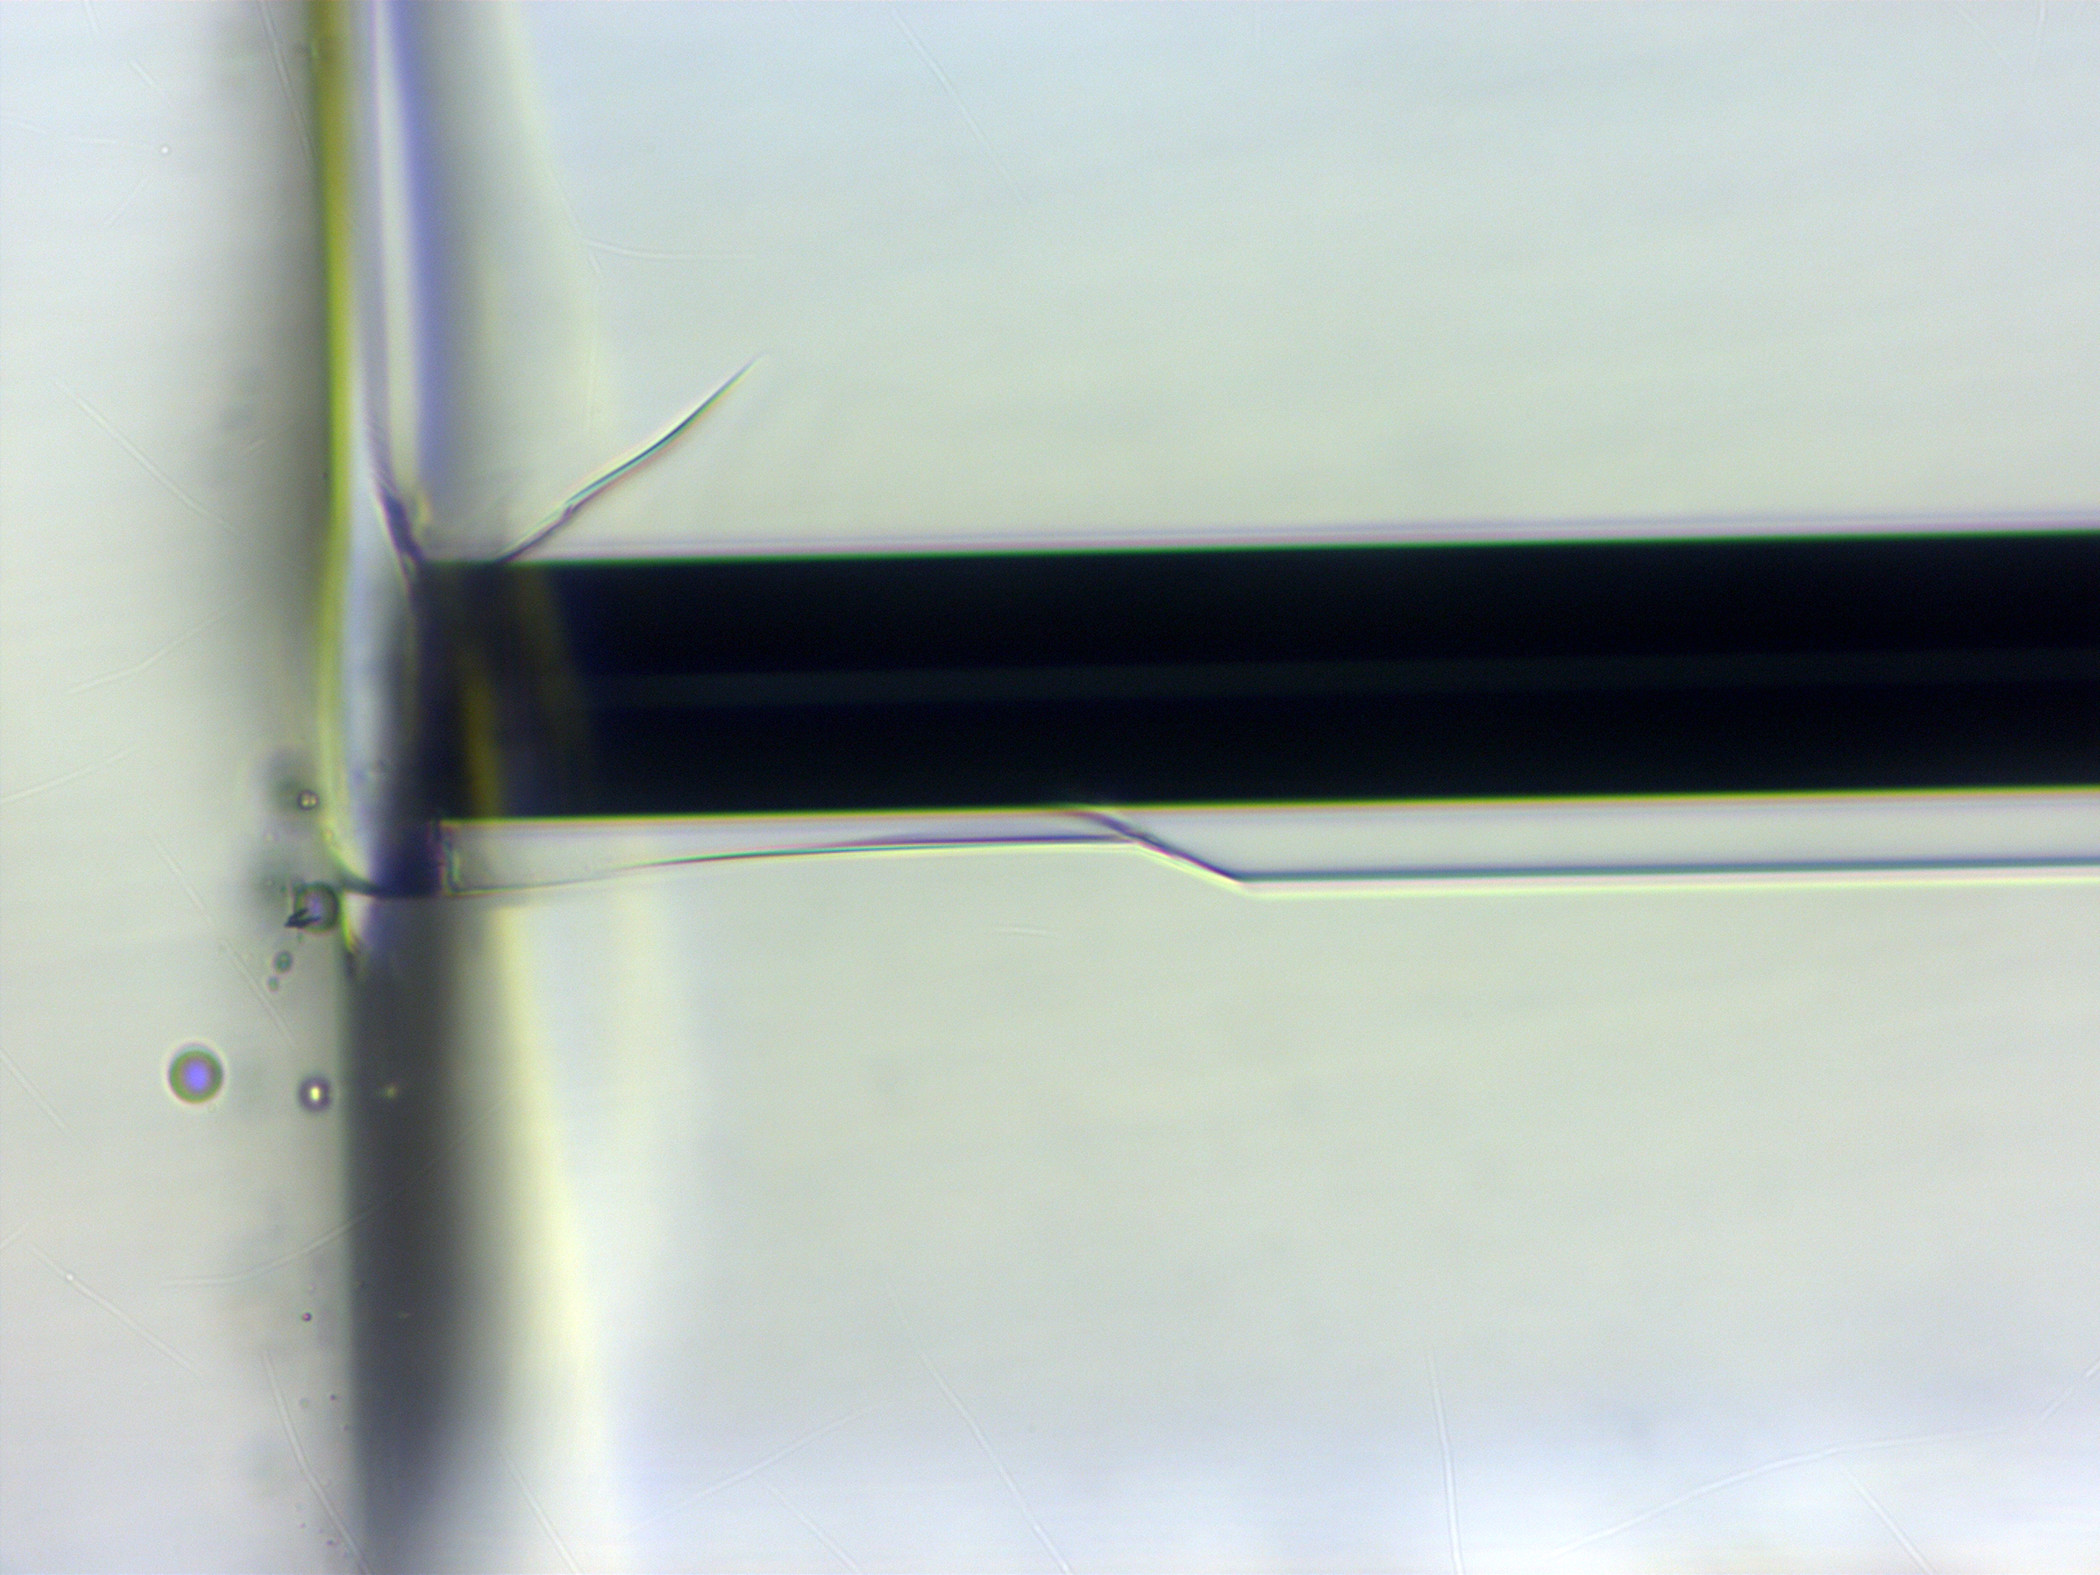
\includegraphics[width=\linewidth]{fig/polishing/parallelcrack2.jpg}
  %\caption{1a}
%  \label{fig:sfig2}
%\end{subfigure}% %blank line makes figures vertical


% \caption{}
%\label{fig:si_sige}
%\end{figure}


\begin{figure}[h]
 %h here H requires float, exactly here, h! overide latex
\centering
\begin{subfigure}{\textwidth}
  \centering
  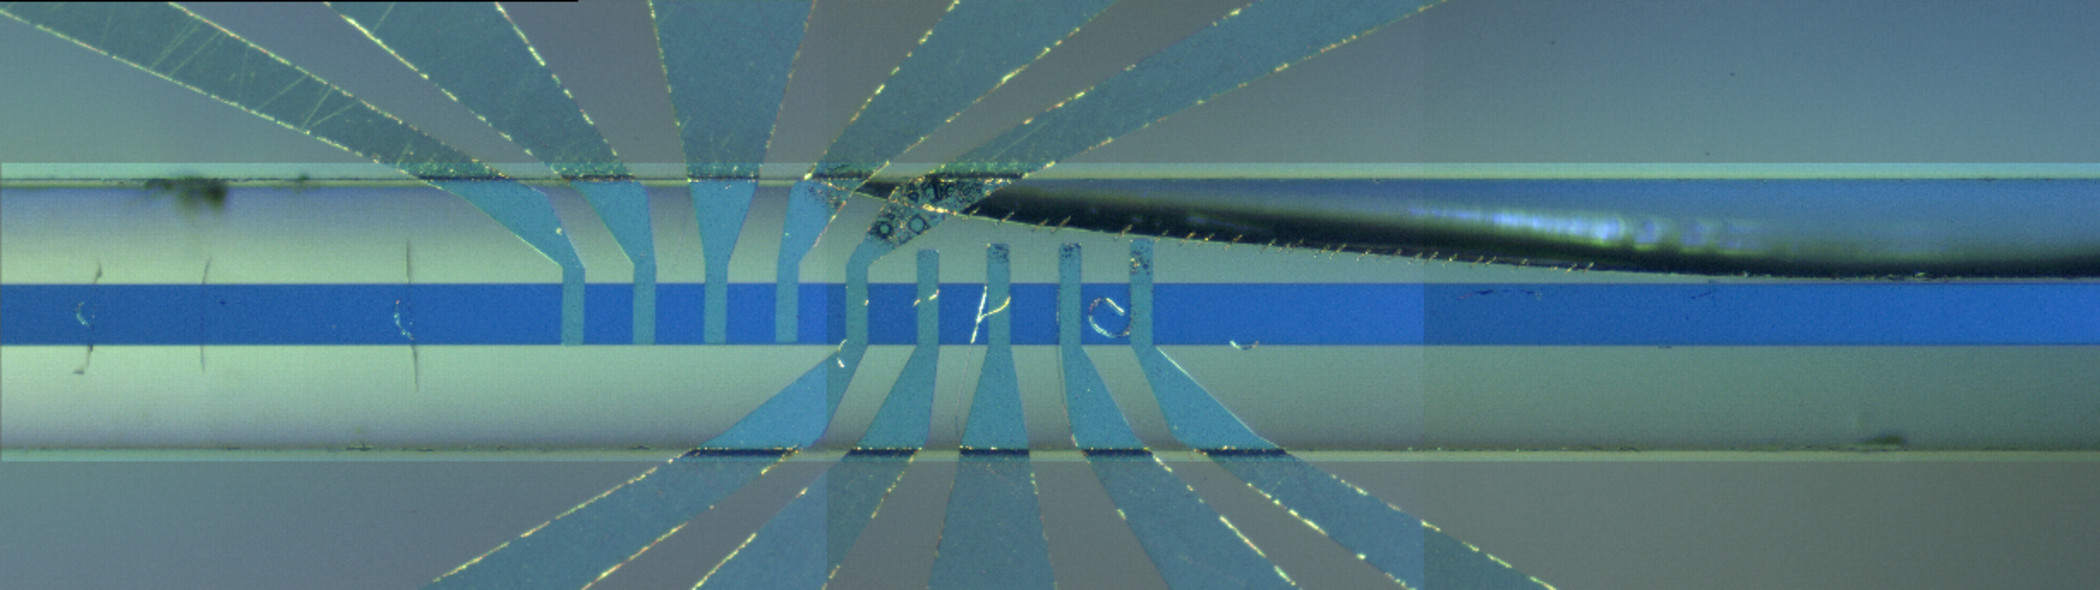
\includegraphics[width=\linewidth]{fig/OA/dd35114_0A--01-1.jpg}
  %\caption{1a}
  \label{fig:sfig1}
\end{subfigure}% %blank line makes figures vertical

\begin{subfigure}{\textwidth}
  \centering
  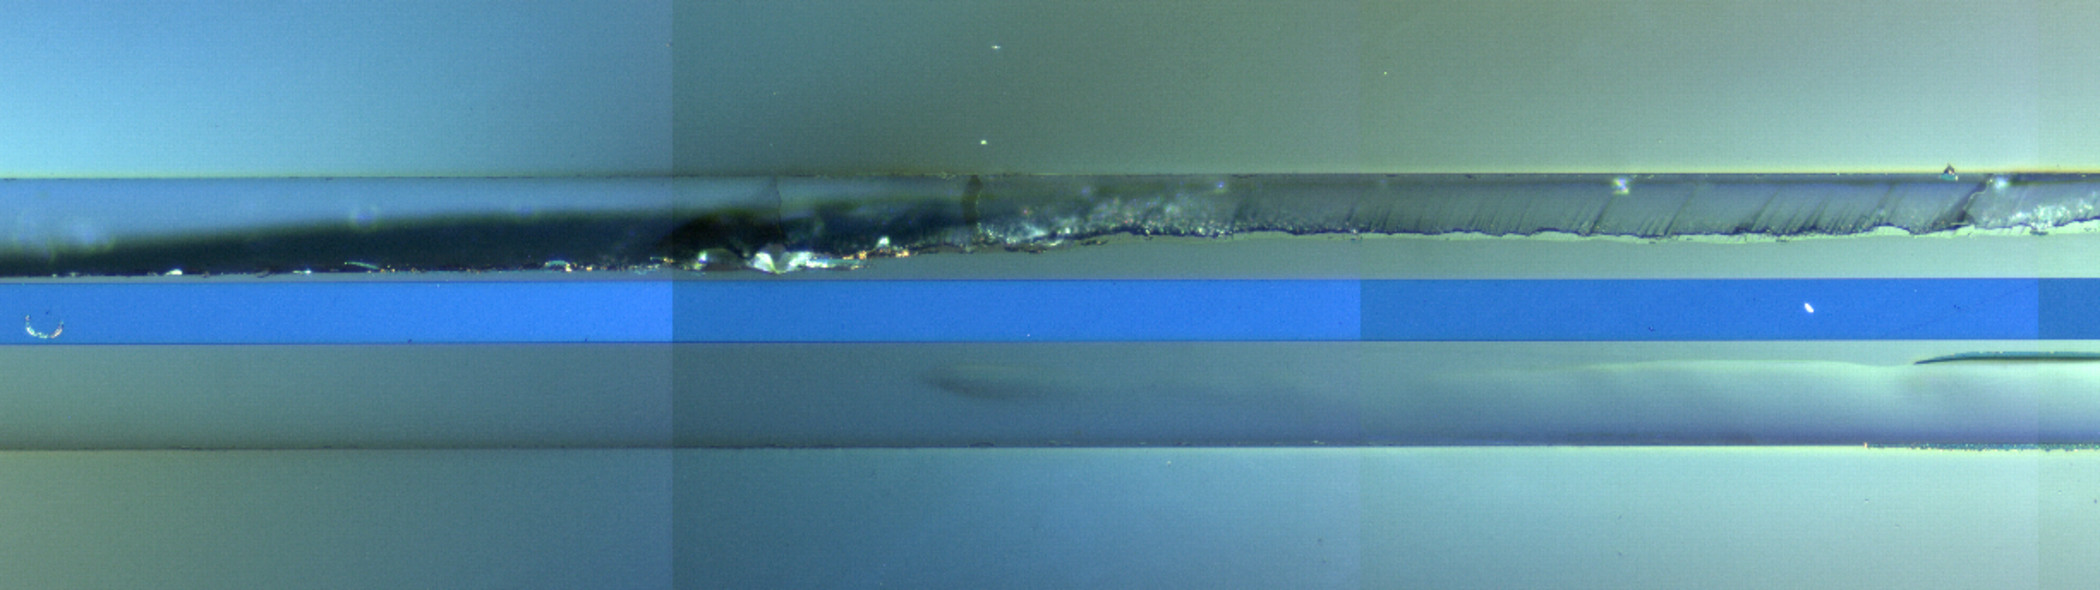
\includegraphics[width=\linewidth]{fig/OA/dd35114_0A--01-2.jpg}
  %\caption{1a}
  \label{fig:sfig2}
\end{subfigure}% %blank line makes figures vertical

\begin{subfigure}{\textwidth}
  \centering
  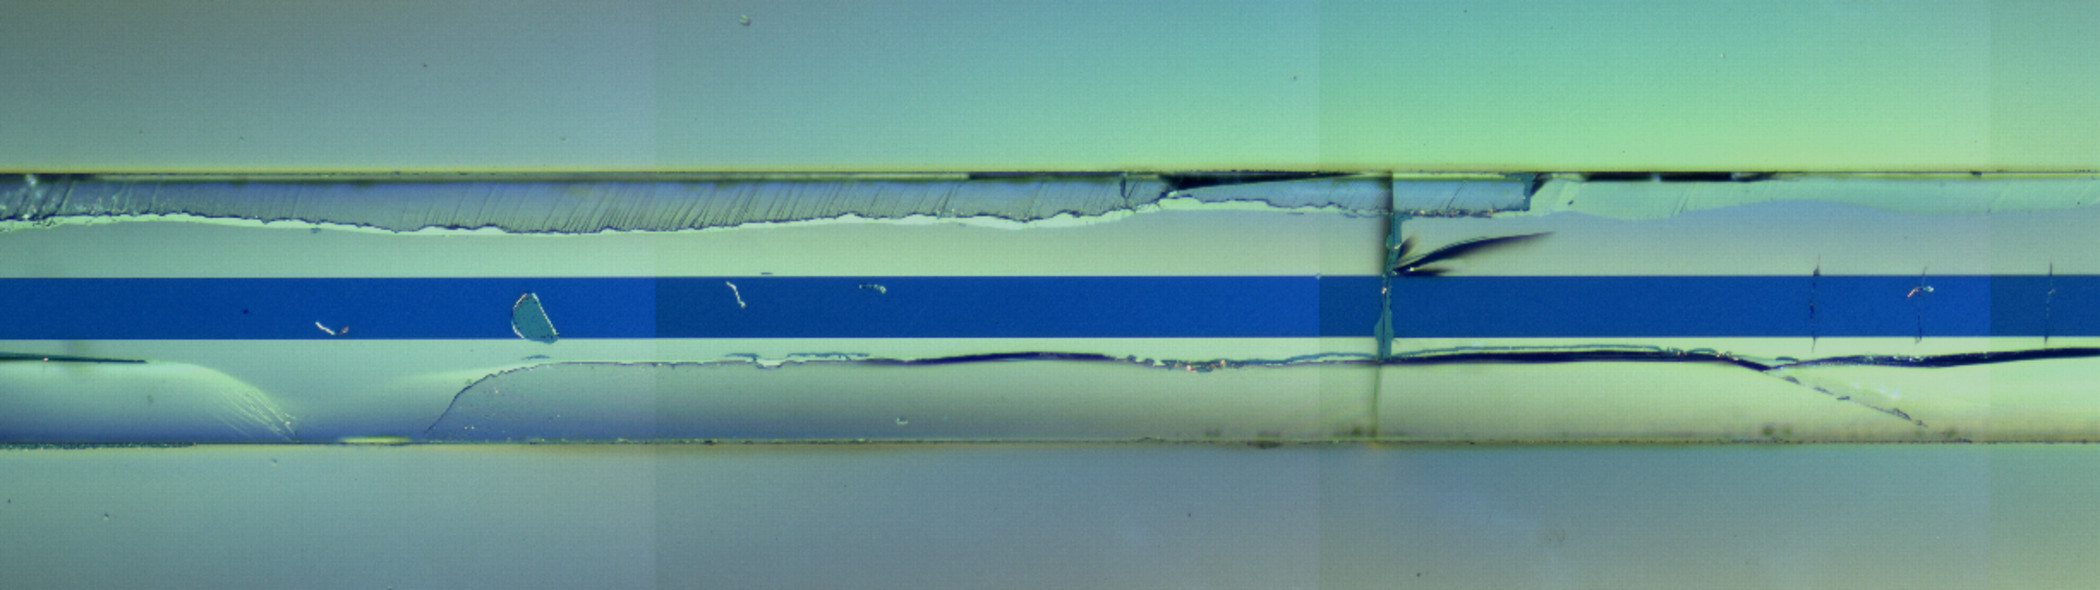
\includegraphics[width=\linewidth]{fig/OA/dd35114_0A--01-3.jpg}
  %\caption{1b}
  \label{fig:sfig3}
\end{subfigure}
\caption{Oven anneal Si fiber Si A taken with a reflected light and polorization filter. Large cracks in the cladding, seem to act as a mechanism to relieve stress, as no cracking is observable in the core for these areas. Note due to image stiching, periodic vertical lines appear. }
\label{fig:si_sige}
\end{figure}


\begin{figure}[h]
 %h here H requires float, exactly here, h! overide latex

\begin{subfigure}{\textwidth}
  \centering
  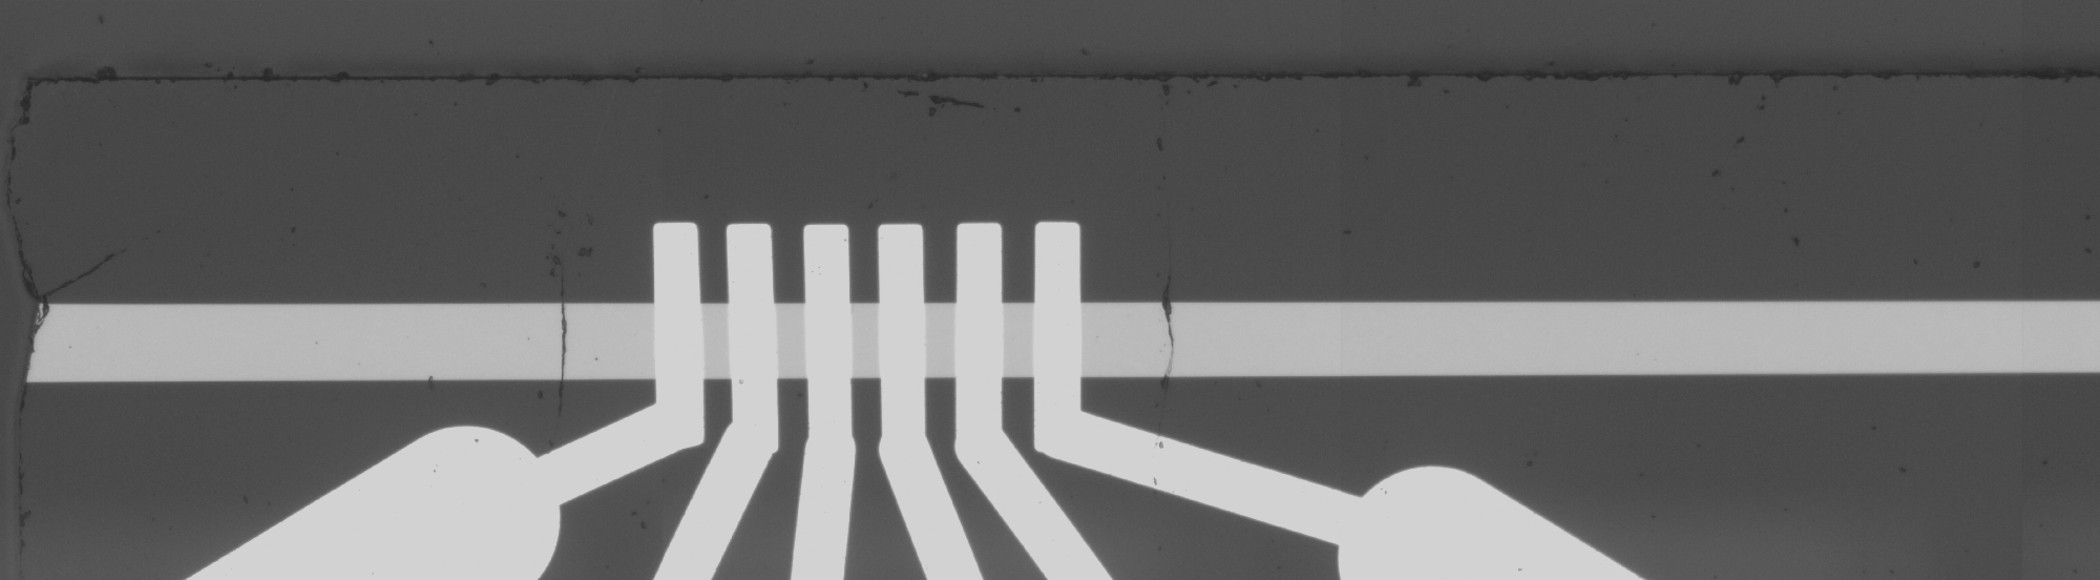
\includegraphics[width=\linewidth]{fig/OA/e944190422_redo-dup1.jpg}
  %\caption{1a}
  \label{fig:sfig1}
\end{subfigure}% %blank line makes figures vertical

\begin{subfigure}{\textwidth}
  \centering
  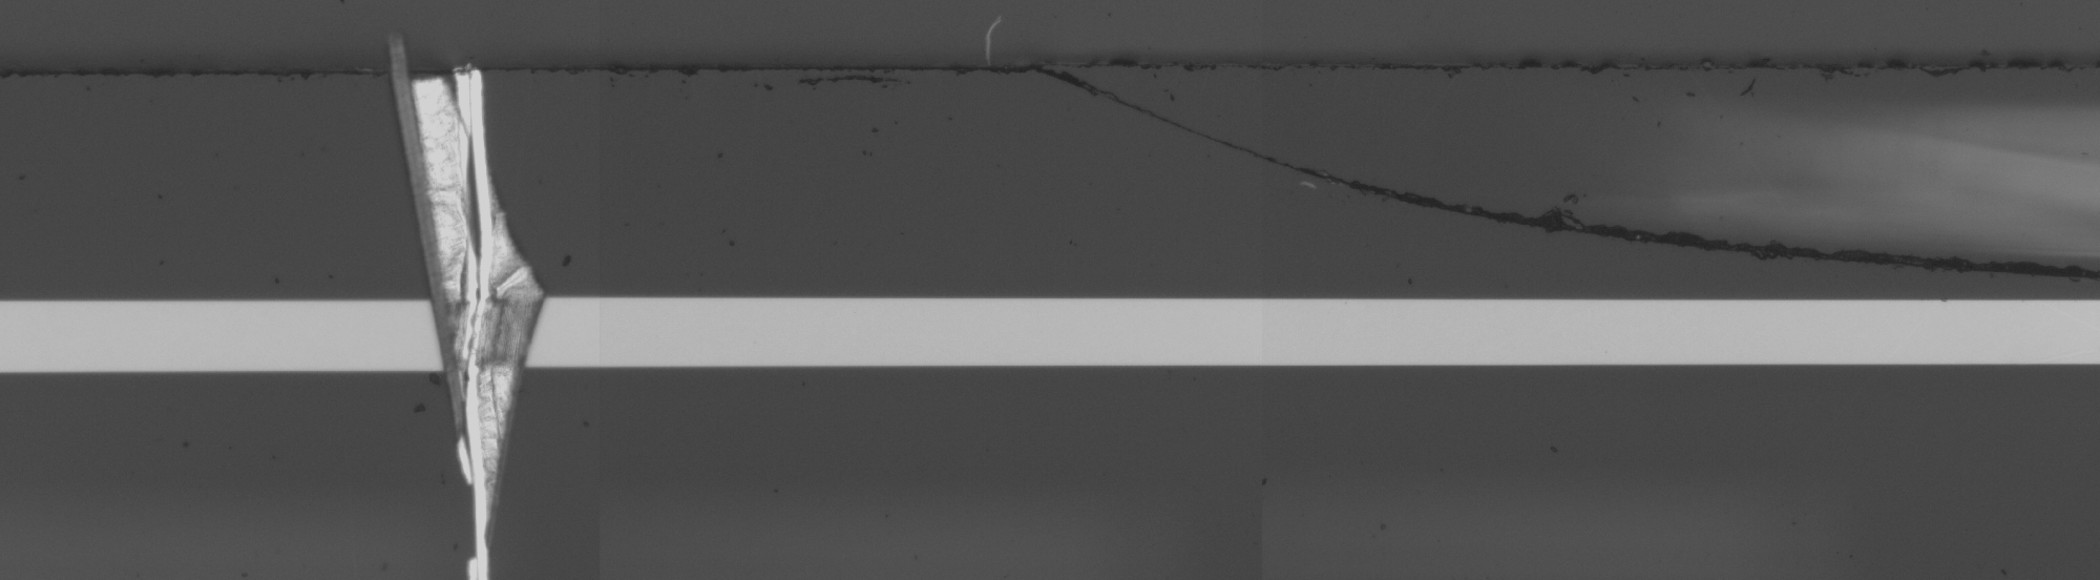
\includegraphics[width=\linewidth]{fig/OA/e944190422_redo-duplicate2.jpg}
  %\caption{1a}
  \label{fig:sfig2}
\end{subfigure}% %blank line makes figures vertical

\caption{Oven annealed Si B fiber showing a large crack-free section of core accompanied by a large crack in the cladding. One crack is seen covered in gold film as a result of an incomplete lift-off process}
\label{fig:si_sige}
\end{figure}


\FloatBarrier
\section{Lithography and Contact Deposition}

\begin{figure}[t!]
    \begin{subfigure}{.5\textwidth}
      \centering
      \includegraphics[width=\linewidth]{fig/Results/DA13118_0422-1_overview.png}
      %\caption{1a}
      
    \end{subfigure}% %blank line makes figures vertical
        \begin{subfigure}{.5\textwidth}
      \centering
      \includegraphics[width=\linewidth]{fig/Results/DA13118_0422-1.png}
      %\caption{1a}
      
    \end{subfigure}% %blank line makes figures vertical
\caption{SiGe C fiber showing a contact pattern used for four point probe measurements. Indentations can be seen in the contact pads left from the pins on the four point probe head. The symmetry in the pattern offers redundancy in the case of a broken contact.}
\label{contact overview}
\end{figure}

\subsection{Lift-off process with man-440}
  The lift-off procedure using man-440 provided a reliable method for contact deposition and contacts were deposited on more than $25$ samples. Ti/Au and Al contacts provided good adhesion to the fiber core, cladding and epoxy, although some peeling of the contact edges could be observed in some cases. Allignment of contacts with the fiber core was easily achieved and allignment with a previous deposition was accurate within a few microns and was useful in some cases for process development purposes and SEM imaging. 
  
  There was some difficulty in finding the correct resist development time. Initially development times were substantially longer than the manufactures value and left resist residues in the developed areas. The available developer was expired by two years, and it was found that the development times changed substantially when a new bottle with the same expiration date (2017??) was used. After several weeks, participate would form in the bottle and the development time would again increase. The developer contains a surfactant to help with the removal of exposed resist. It appears that the resist left more residues as the developer aged, possibly indicating a reduction in the cleaning action of the surfactant. It was found that the residue increased with increasing development time, and a "halo" could be seen around the contacts as seen in figure \ref{fig:residue}. Past the minimum development time the undercut increases and it appears that some delamination of the resist occurs. The developer may not have sufficient circulation in these confined areas to cleanly remove the resist. A fresh developer could improve the results as well as the  use of HDMS as an adhesion layer. As there is some relief between the fiber and the epoxy, resist thickness increases adjacent to the fiber similar to that seen in figure \ref{mrdwl-si}. In order to fully develop the thicker resist, it is necessary to over-develop thinner areas, thus it is not possible to fully control the development at the fiber core. For this reason, polishing times should be minimized to avoid excessive relief. 
  
  %%fiber swelling?? %%
  %%fiber interface? profilometry?
  
  The use of a plasma-ash was successful in removing these residues. The removal rate of the cross-linked resist was low, and measurement with a stylus profilometer showed no noticable change in resist height for the cleaning parameters used. It would be worth investigating longer cleaning times to see if there is any affect on contact resistance. 
 
 \begin{figure}[h]
     \centering
     \begin{subfigure}{.47\textwidth}
       \begin{tikzpicture}[x=1cm,y=1cm]
      \node[anchor=south west,inner sep=0] (image) at (0,0) {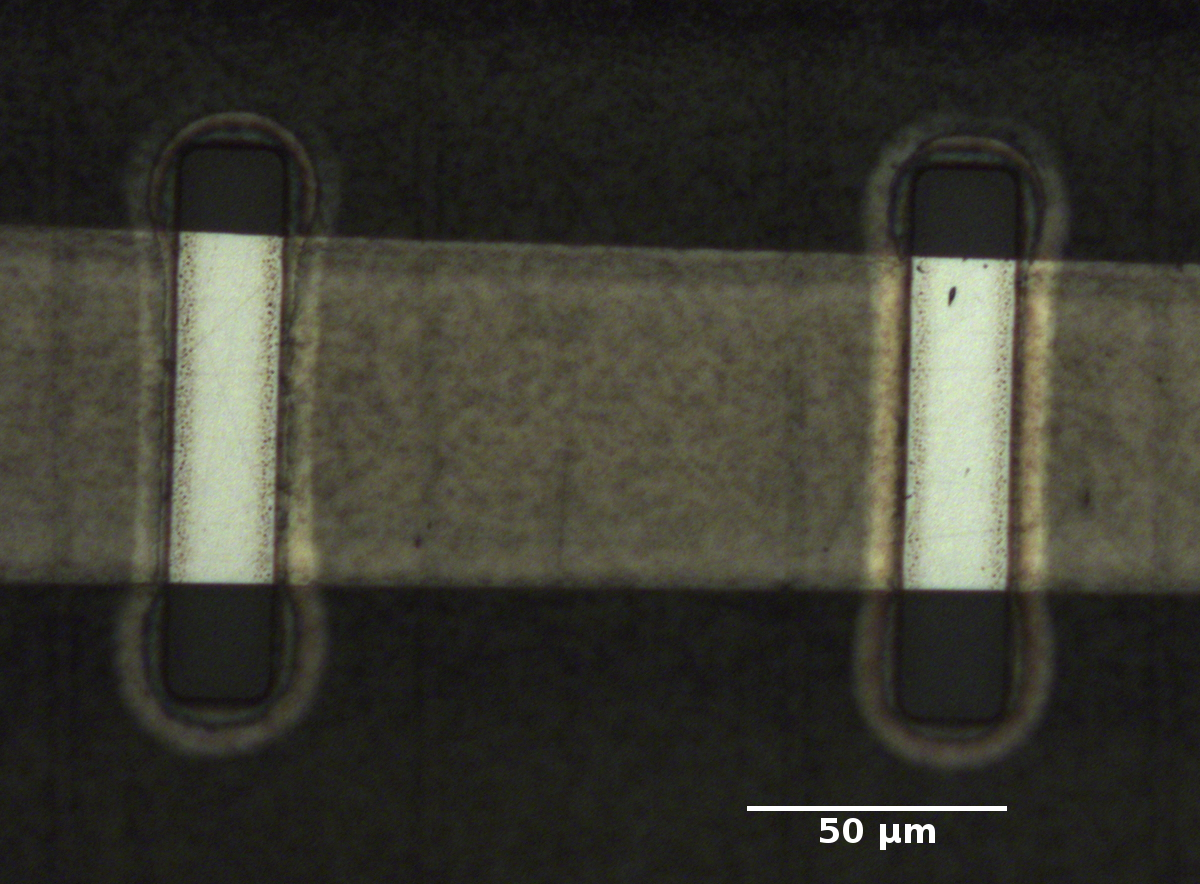
\includegraphics[ width=\linewidth]{fig/Results/scumming2.png}};
       \begin{scope}[x={(image.south east)},y={(image.north west)}]
        \draw[white,thick,->](.26,.64) -- (.23,.6);
         \node[right,white] at (.26,.64) {\large resist residue };
        \end{scope}
  \end{tikzpicture}
  \end{subfigure}
    \begin{subfigure}{.47\textwidth}
    \centering
    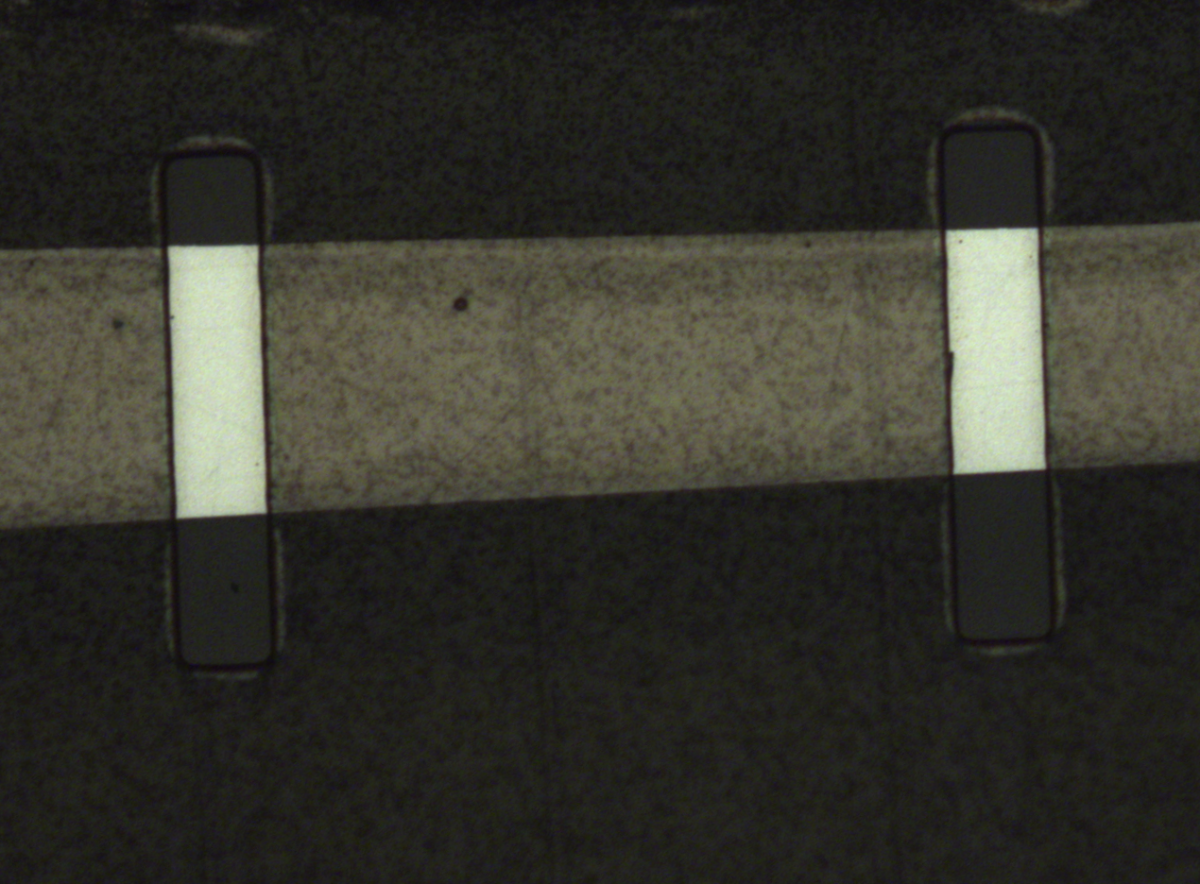
\includegraphics[width=\linewidth]{fig/Results/scumming3_resize.png}
  \end{subfigure}
\caption{Developed man-440 resist showing resist residue with longer development time (left) and clean development (right). }
\label{fig:residue}
 \end{figure}
 \FloatBarrier
 
 \subsection{Permanent Resist Underlayer}
 
 The test sample using an mr-DWL-5 as a permanent layer and man-440 for lift-off is shown in figure \ref{mrdwl-si}. The most important result from this test is that although man-440 is $\SI{4.1}{\micro\meter}$ it is able to form a continuous layer over the $\SI{5}{\micro\meter}$mr-DWL-5 step edge. The resist thickness increases close to the step edge, and is thickest between the two mr-DWL structures. This area between the structures will represent the exposed fiber core flanked by mr-DWL, and suggests that man-440 will pool in this area will create a thick enough resist layer over the edge to perform liftoff. 
 
 Liftoff was tested using a resist geometry resembling that used for a fiber (figure \ref{mrdwl-butterfly})and Ti/Au contacts ($5/100 \si{\nano\meter}$ ). The hard baked mr-DWL resist proved very stable and showed no deterioration or delamination after sonication in acetone. The contacts showed good adhesion to the mr-DWL resist, however it was found that there was no electrical conductivity between the contacts. An additional $100 \si{\nano\meter}$ was sputtered onto each step edge face using the small cressington 208 HR B  sputter coater with the sample tilted $\ang{45}$. After this additional deposition, there was conductivity between the contacts. This suggests that e-beam deposition does not provide enough coverage of the vertical mr-DWL faces.
 \begin{figure}
    \centering
    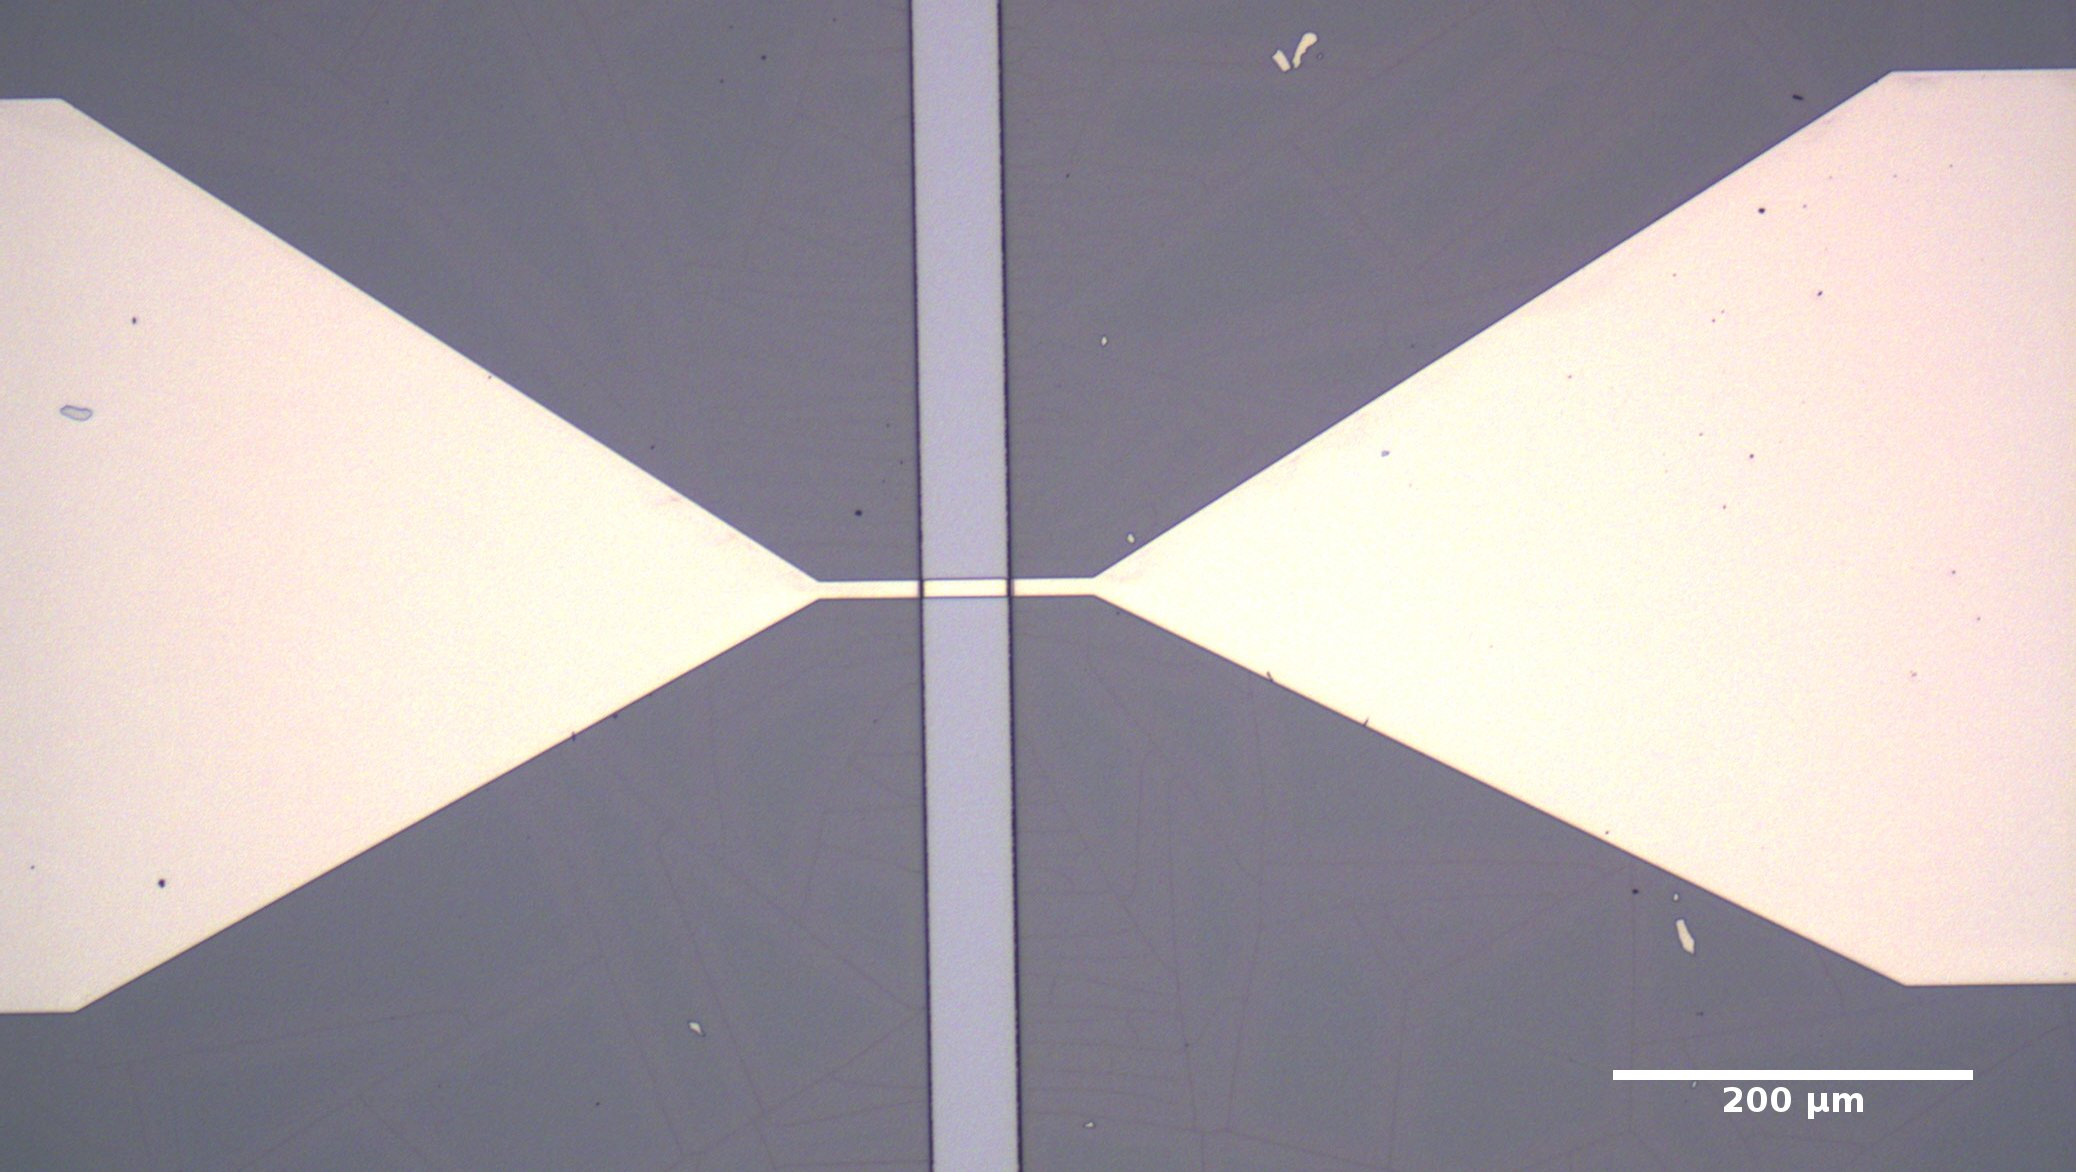
\includegraphics[width=.8\textwidth]{fig/Results/mr-dwl_test_butterfly.jpg}
    \caption{A test sample of Ti/Au contacts over an mr-DWL resist layer. The strip in the middle is the Si substrate coated with mr-DWL on either side. Only one contact pair is shown of many deposited on the sample}
    \label{mrdwl-optic}
\end{figure}

\begin{figure}
    \centering
    \includegraphics[width=.8\textwidth]{fig/Results/mrdwl_optical.png}
    \caption{Contacts on a fiber using mr-DWL underlayer. The image was taken while tilting the sample thus coverage of the step edge can be seen. The mr-DWL is transparent and a crack can be seen underneath the leftmost contact.}
    \label{mrdwl-butterfly}
\end{figure}

 \begin{figure}[htb]
 %h here H requires float, exactly here, h! overide latex
\centering
\begin{subfigure}{\textwidth}
  \centering
  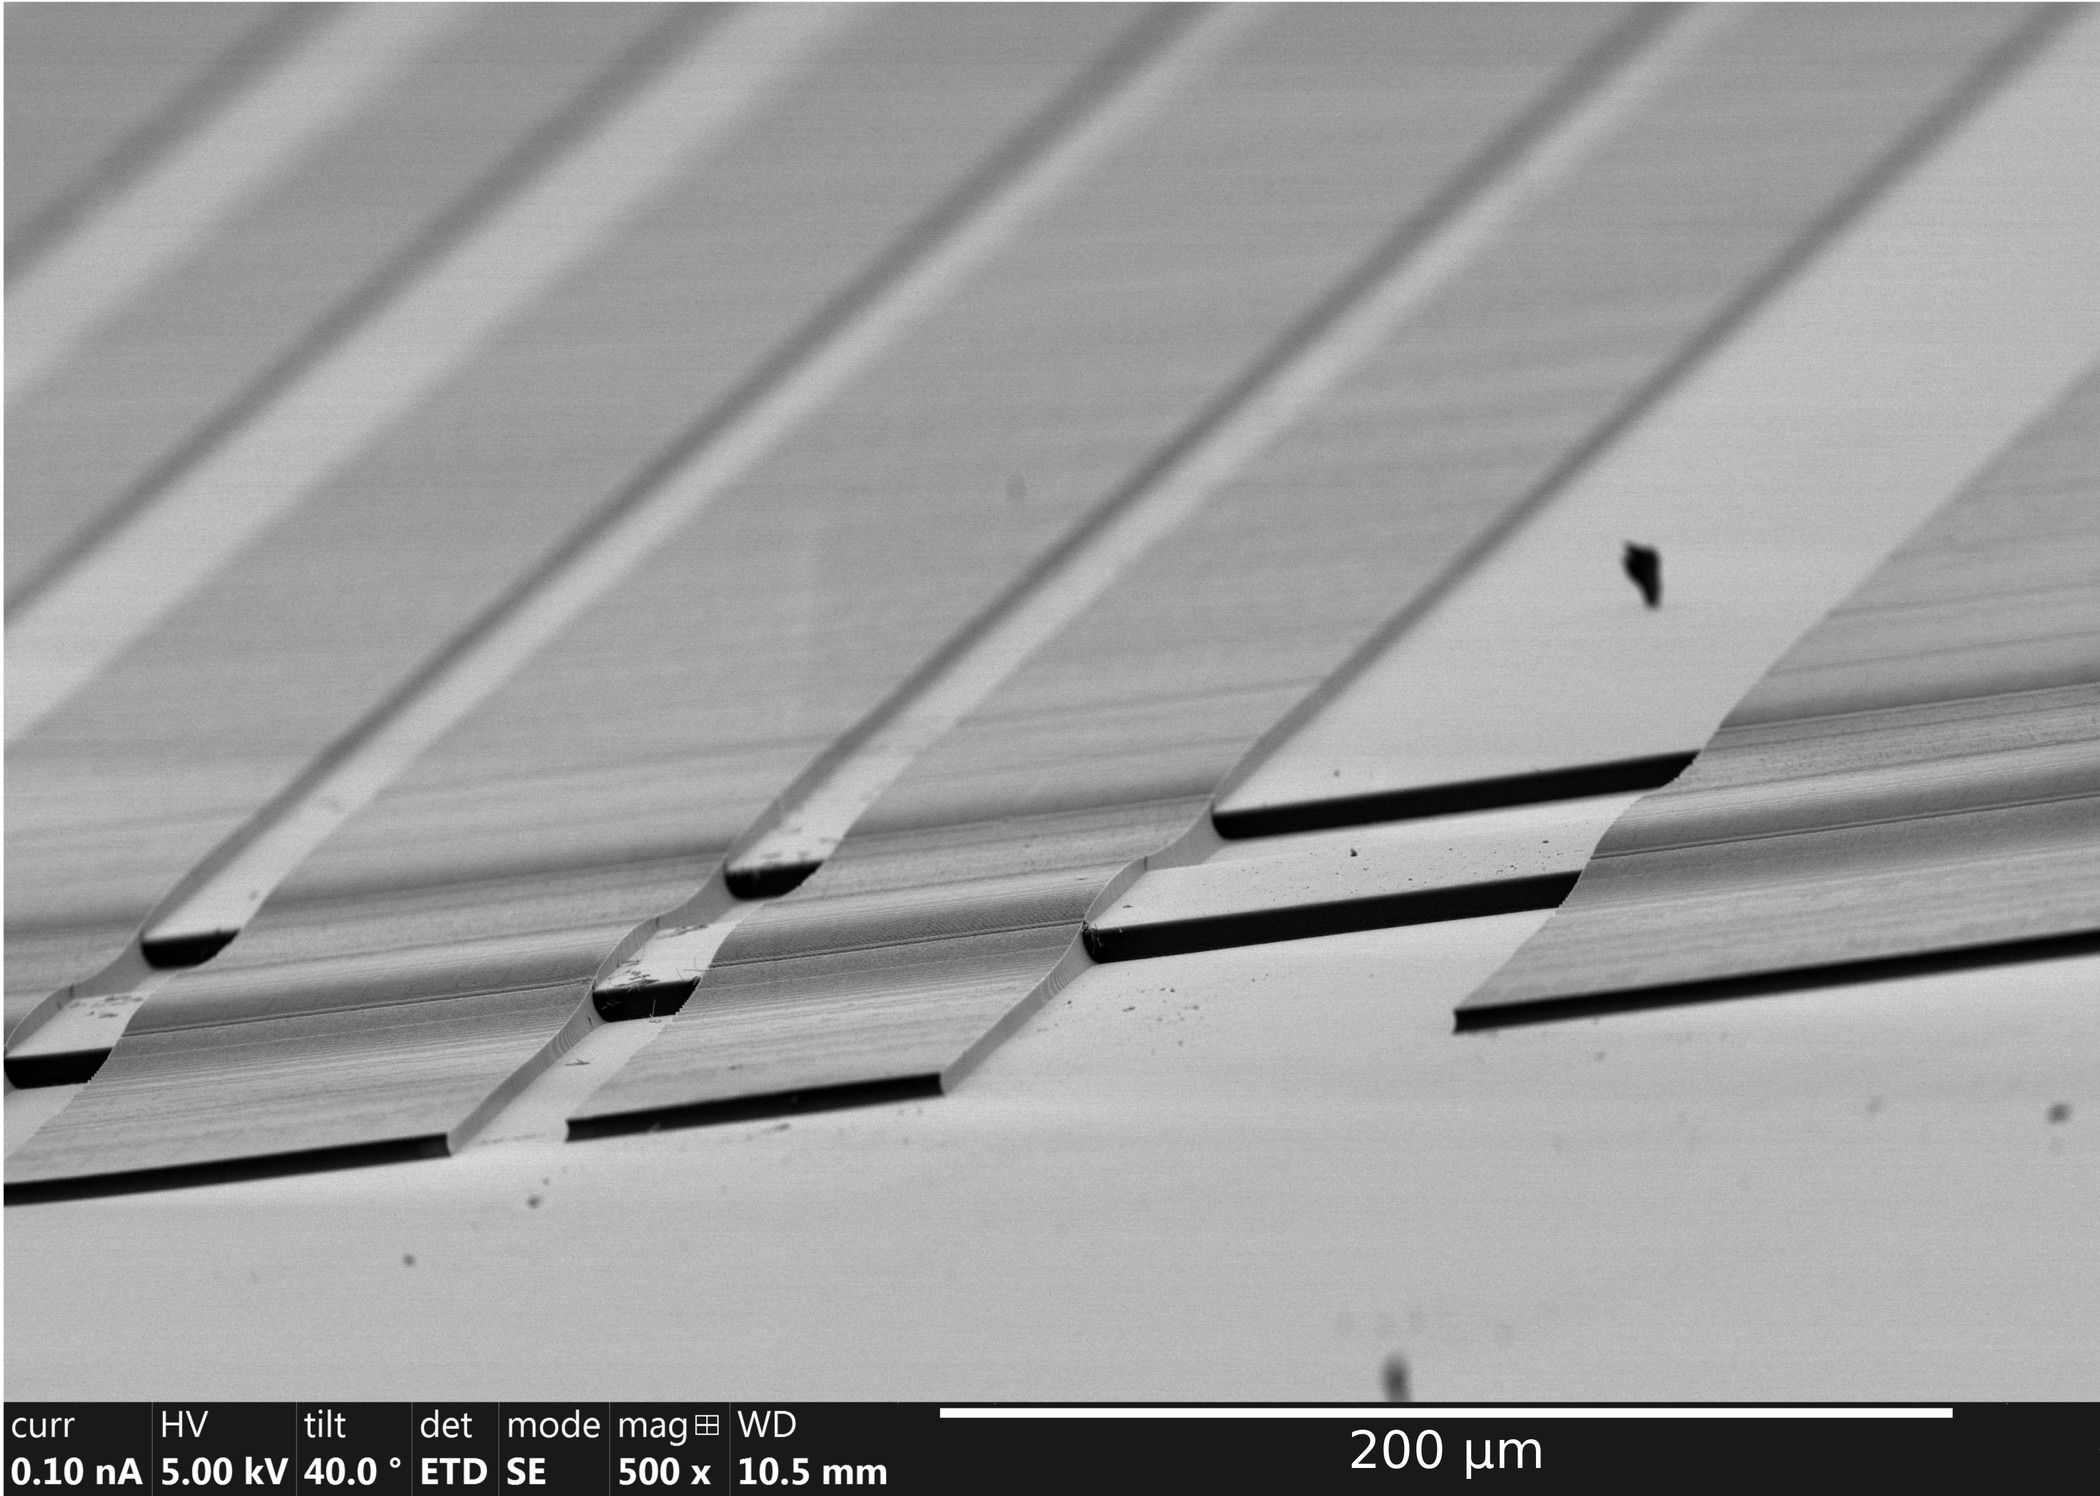
\includegraphics[width=\linewidth]{fig/mr-DWL/sem_mr-dwl-2.jpg}
  %\caption{1a}
 
\end{subfigure}% %blank line makes figures vertical

\begin{subfigure}{\textwidth}
  \centering
  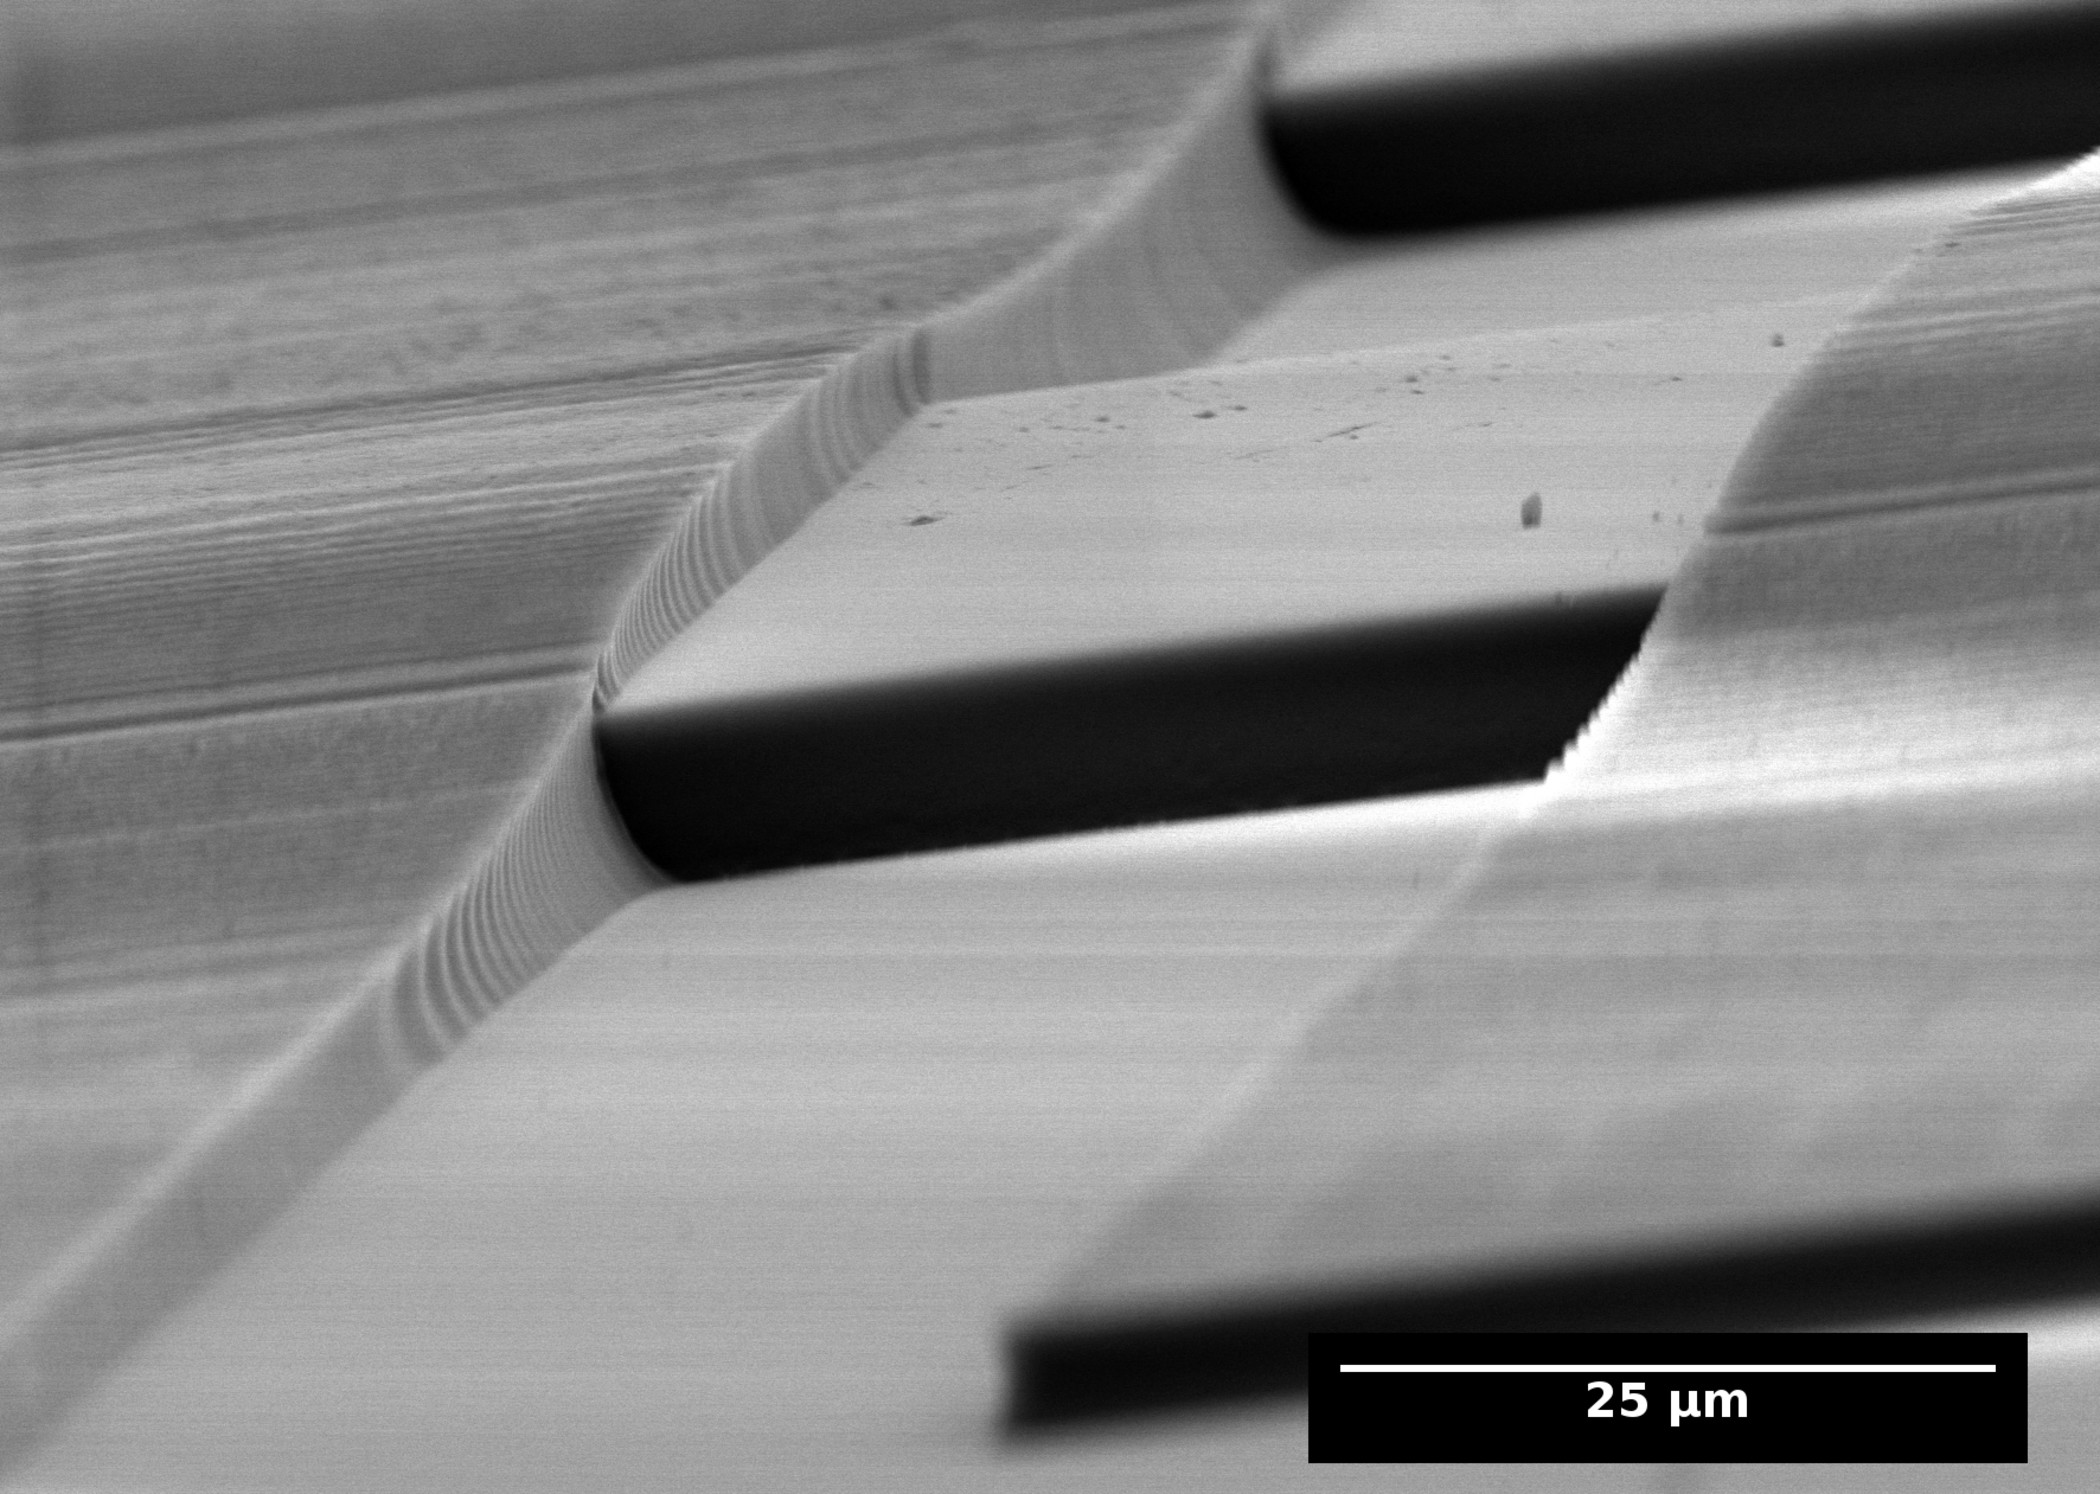
\includegraphics[width=\linewidth]{fig/mr-DWL/sem_mr-dwl_zoom4.jpg}
  %\caption{1b}
 
\end{subfigure}
\caption{$5um$ mr-DWL resist structures coated with a $4um$ man440 layer, demonstrating the possibility of patterning resist structures over a high step edge. }
\label{mrdwl-si}
\end{figure}
 Repeating the procedure on a polished fiber sample gave similar results. There was no electrical conductivity before sputtering of an additional $100 \si{\nano\meter}$ Au with a sputter coater. The mr-DWL succesfully covered a large crack in the fiber cladding, as seen in figure \ref{mrdwl_onfiber}. The surface of the resist became distorted above the crack, but this did not cause any discontinuity in the contacts. Figure \ref{mrdwl_step} shows a close up of the step edge.  It can be seen that the vertical mr-DWL surface has been coated but it appears to have a wavy texture. This may be due to poor adhesion of the deposited layer, as it was only possible to deposit the Ti adhesion layer via e-beam and thus this surface would not be coated. It may be also originate from some texture of the sidewalls themselves. The exposure is not always even throughout the thickness of the resist due to interference with light reflected from the surface. It should be noted that in order to image these samples in the SEM with a conductive coating without sacrificing the sample, a second layer of man-440 has been applied after contact deposition. 
 
This method shows promise for allowing hall measurement of fibers or four point measurements of heavily cracked fibers when micromanipulators are not available. Currently a new e-beam is being installed at ntnu nanolab which will allow for tilting of the sample during evaporation. This should lead to even coating of the resist step edge. Optimization of the mr-DWL recipe is also necessary as the resist did no always develop cleanly. A longer development time, more thorough rinse in IPA and a plasma ash can all be used to improve the development.

 








 
  
\begin{figure}[h!]
 %h here H requires float, exactly here, h! overide latex
\centering
\begin{subfigure}{\textwidth}
  \centering
  \begin{tikzpicture}[x=1cm,y=1cm]
 
    \node[anchor=south west,inner sep=0] (image) at (0,0) {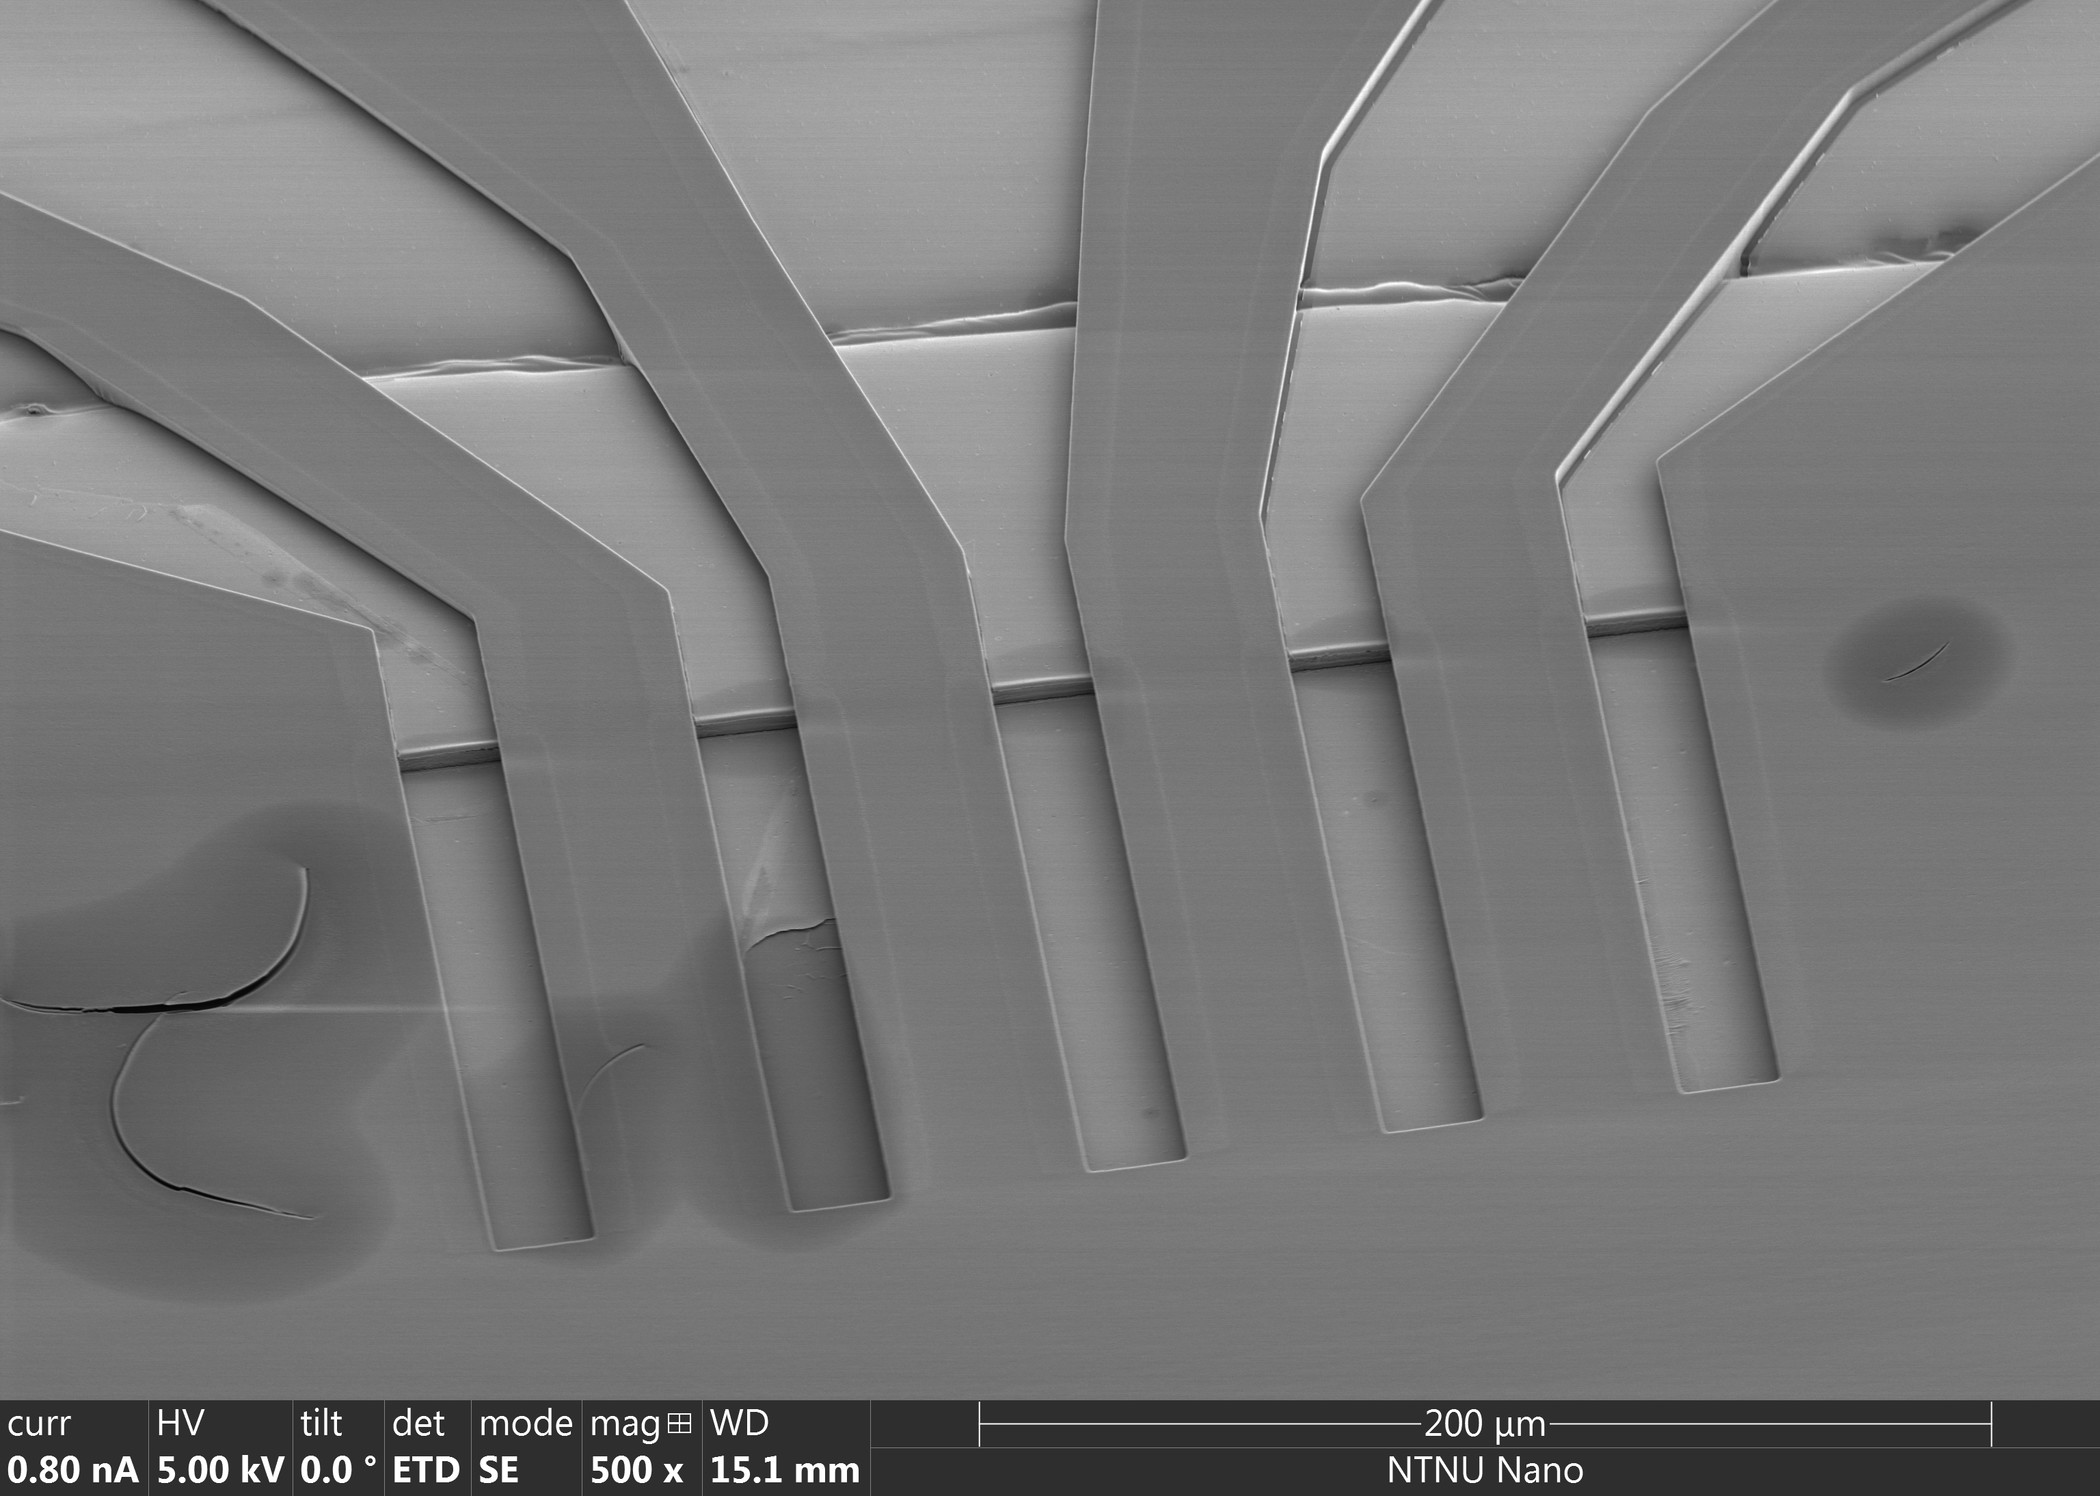
\includegraphics[ width=\textwidth]{fig/mr-DWL/mb_25_overview_002.jpg}};
   
    \begin{scope}[x={(image.south east)},y={(image.north west)}]
    
        %delete
        %\draw[help lines,xstep=.02,ystep=.02] (0,0) grid (1,1); 
        %\foreach \x in {0,1,...,9} { \node [anchor=north] at (\x/10,0) {0.\x}; }
        %\foreach \y in {0,1,...,9} { \node [anchor=east] at (0,\y/10) {0.\y}; }
        %delete
        
         \draw[white,thick,->](.43,.83) -- (.45,.79);
         \node[right,white] at (.38,.86) {\large crack };
          \node[above,white] at (.42,.92) {\large mr-DWL};
           \node[above,white] at (.24,.92) {\large man-440};
        % \node[right,white, ] at (0,.1) {\Large Michael babe};
         %\node[right,yellow] at (.7,.7) {\textbf{\Huge Piggie}};
         %\draw[white,ultra thick,rounded corners] (.5,.3) rectangle (.6,.2);
         \draw[white, thick, dotted](0,.12) -- (1,.3);
        \draw[white, thick, dotted](0,.44) -- (1,.6); 
         \draw[white,thick,->](.9,.45) -- (.88,.54);
         \draw[white,thick,->](.9,.40) -- (.88,.3);
        \node[above,white] at (.9,.4) {\large fiber core};
     \end{scope}
  \end{tikzpicture}
  
  %\caption{1a}
  
\end{subfigure}% %blank line makes figures vertical

\begin{subfigure}{\textwidth}
  \centering
    \begin{tikzpicture}[x=1cm,y=1cm]
 
    \node[anchor=south west,inner sep=0] (image) at (0,0) {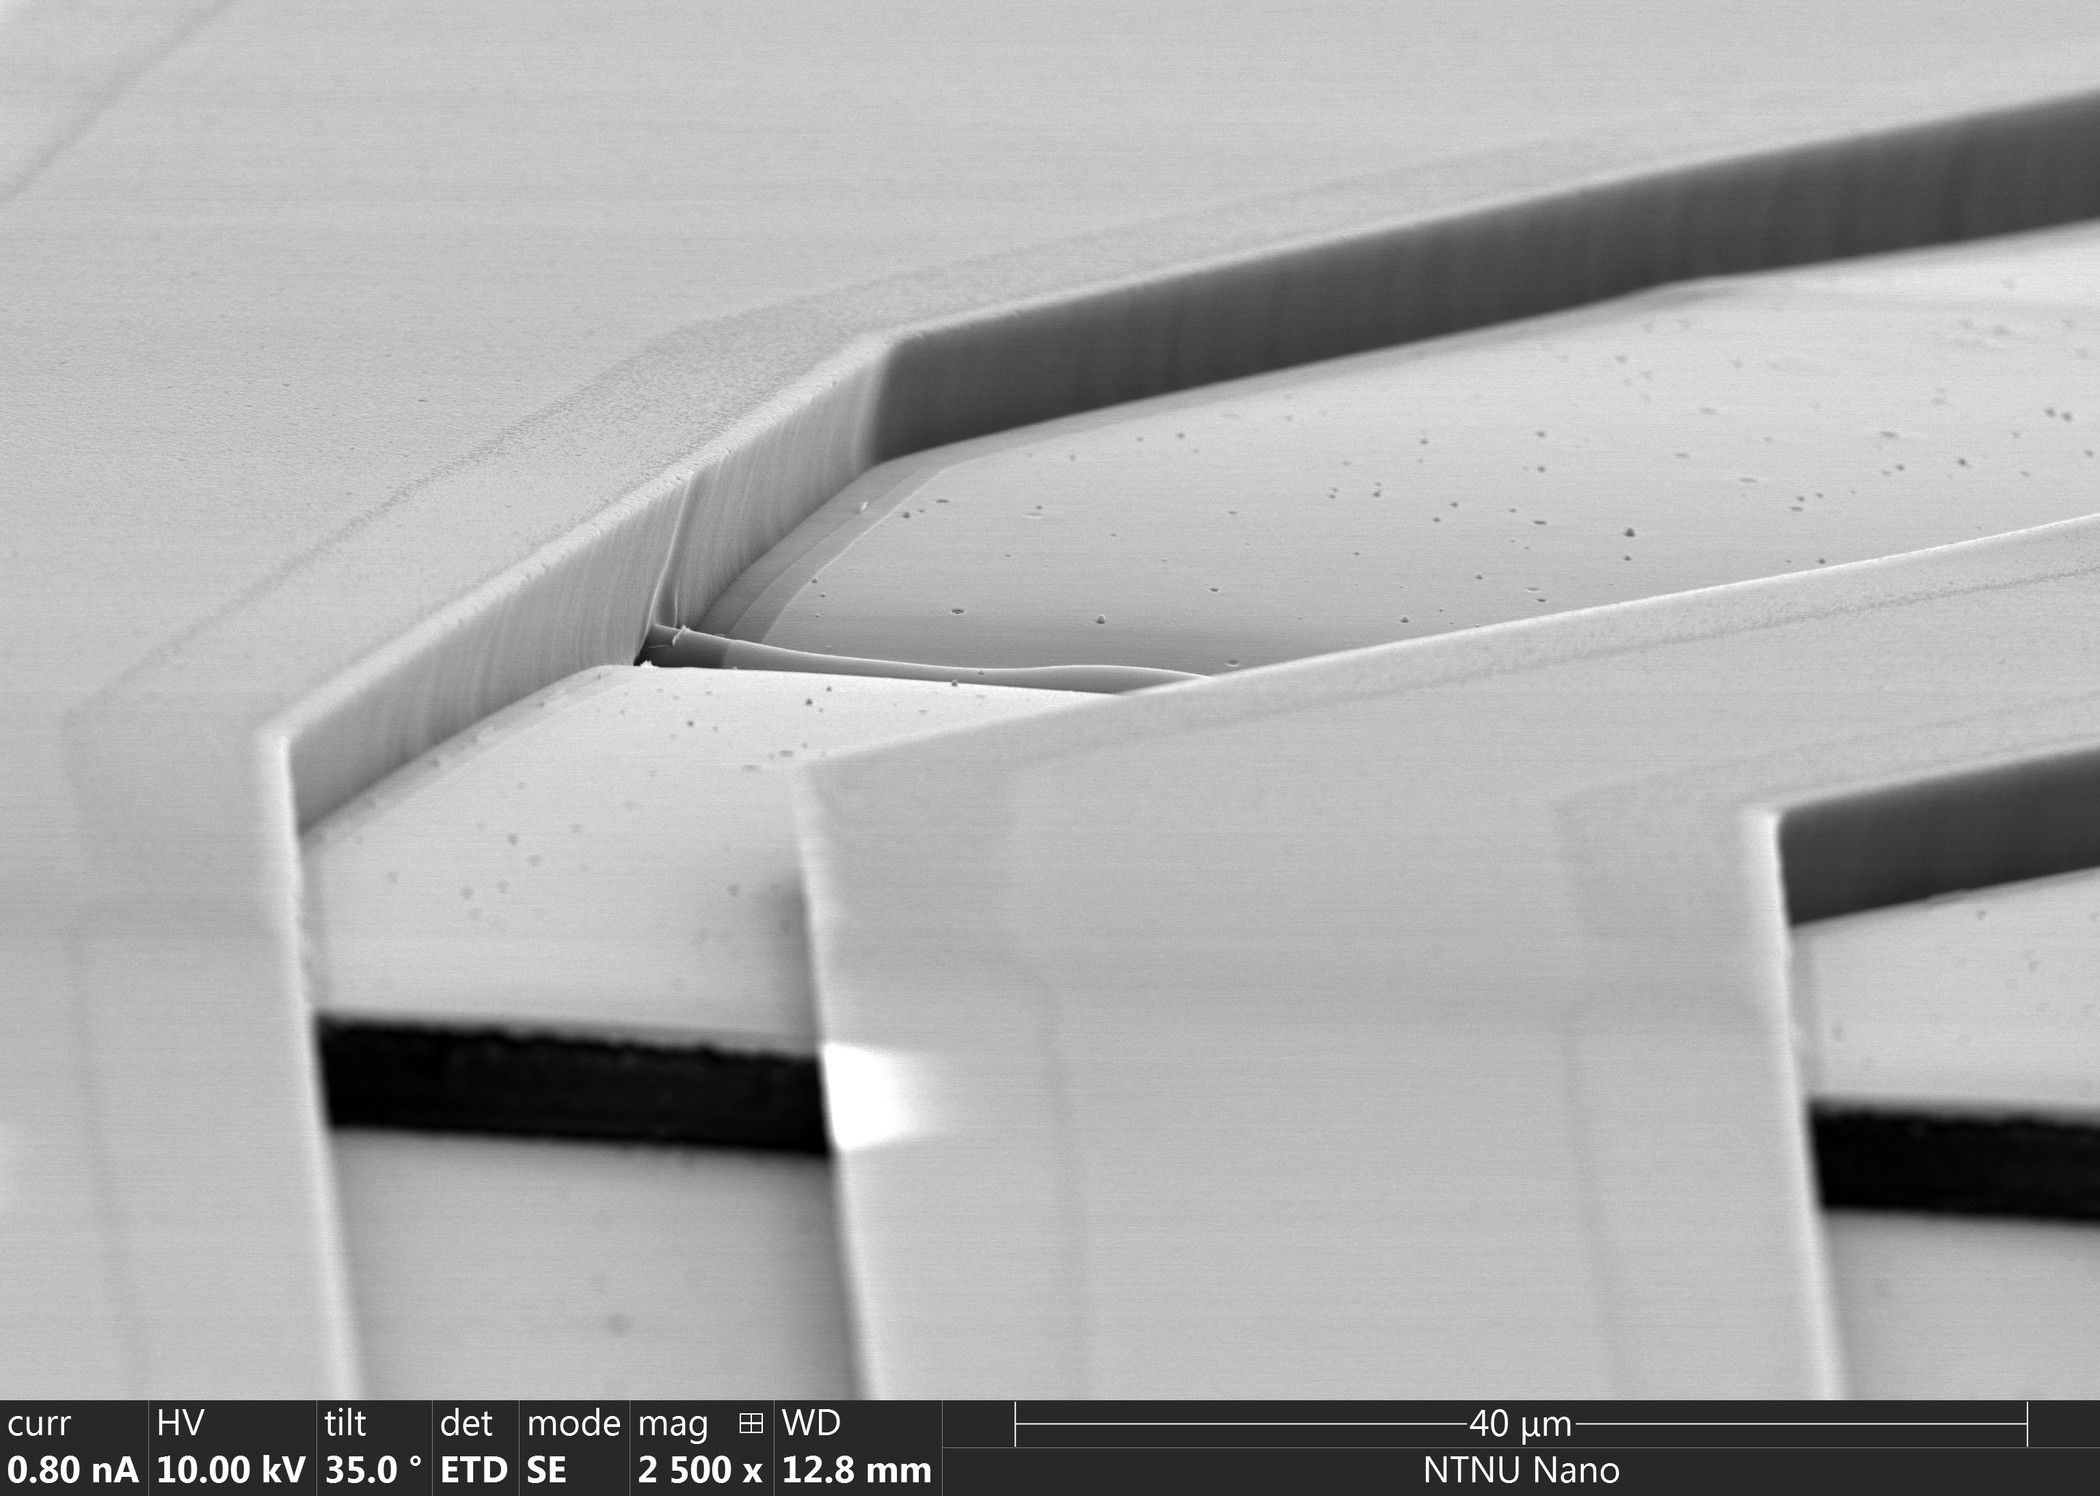
\includegraphics[ width=\textwidth]{fig/mr-DWL/mb_25_step_004.jpg}};
   
    \begin{scope}[x={(image.south east)},y={(image.north west)}]
    
        %delete
        %\draw[help lines,xstep=.02,ystep=.02] (0,0) grid (1,1); 
        %\foreach \x in {0,1,...,9} { \node [anchor=north] at (\x/10,0) {0.\x}; }
        %\foreach \y in {0,1,...,9} { \node [anchor=east] at (0,\y/10) {0.\y}; }
        %delete
        
         \draw[red,thick,->](.5,.6) -- (.47,.56);
         \node[right,red] at (.5,.64) {\large crack };
         \node[above,red] at (.8,.7) {\large mr-DWL};
         \node[above,red] at (.2,.85) {\large man-440};
        % \node[right,red, ] at (0,.1) {\Large Michael babe};
         %\node[right,yellow] at (.7,.7) {\textbf{\Huge Piggie}};
         %\draw[red,ultra thick,rounded corners] (.5,.3) rectangle (.6,.2);
       
     \end{scope}
  \end{tikzpicture}
  %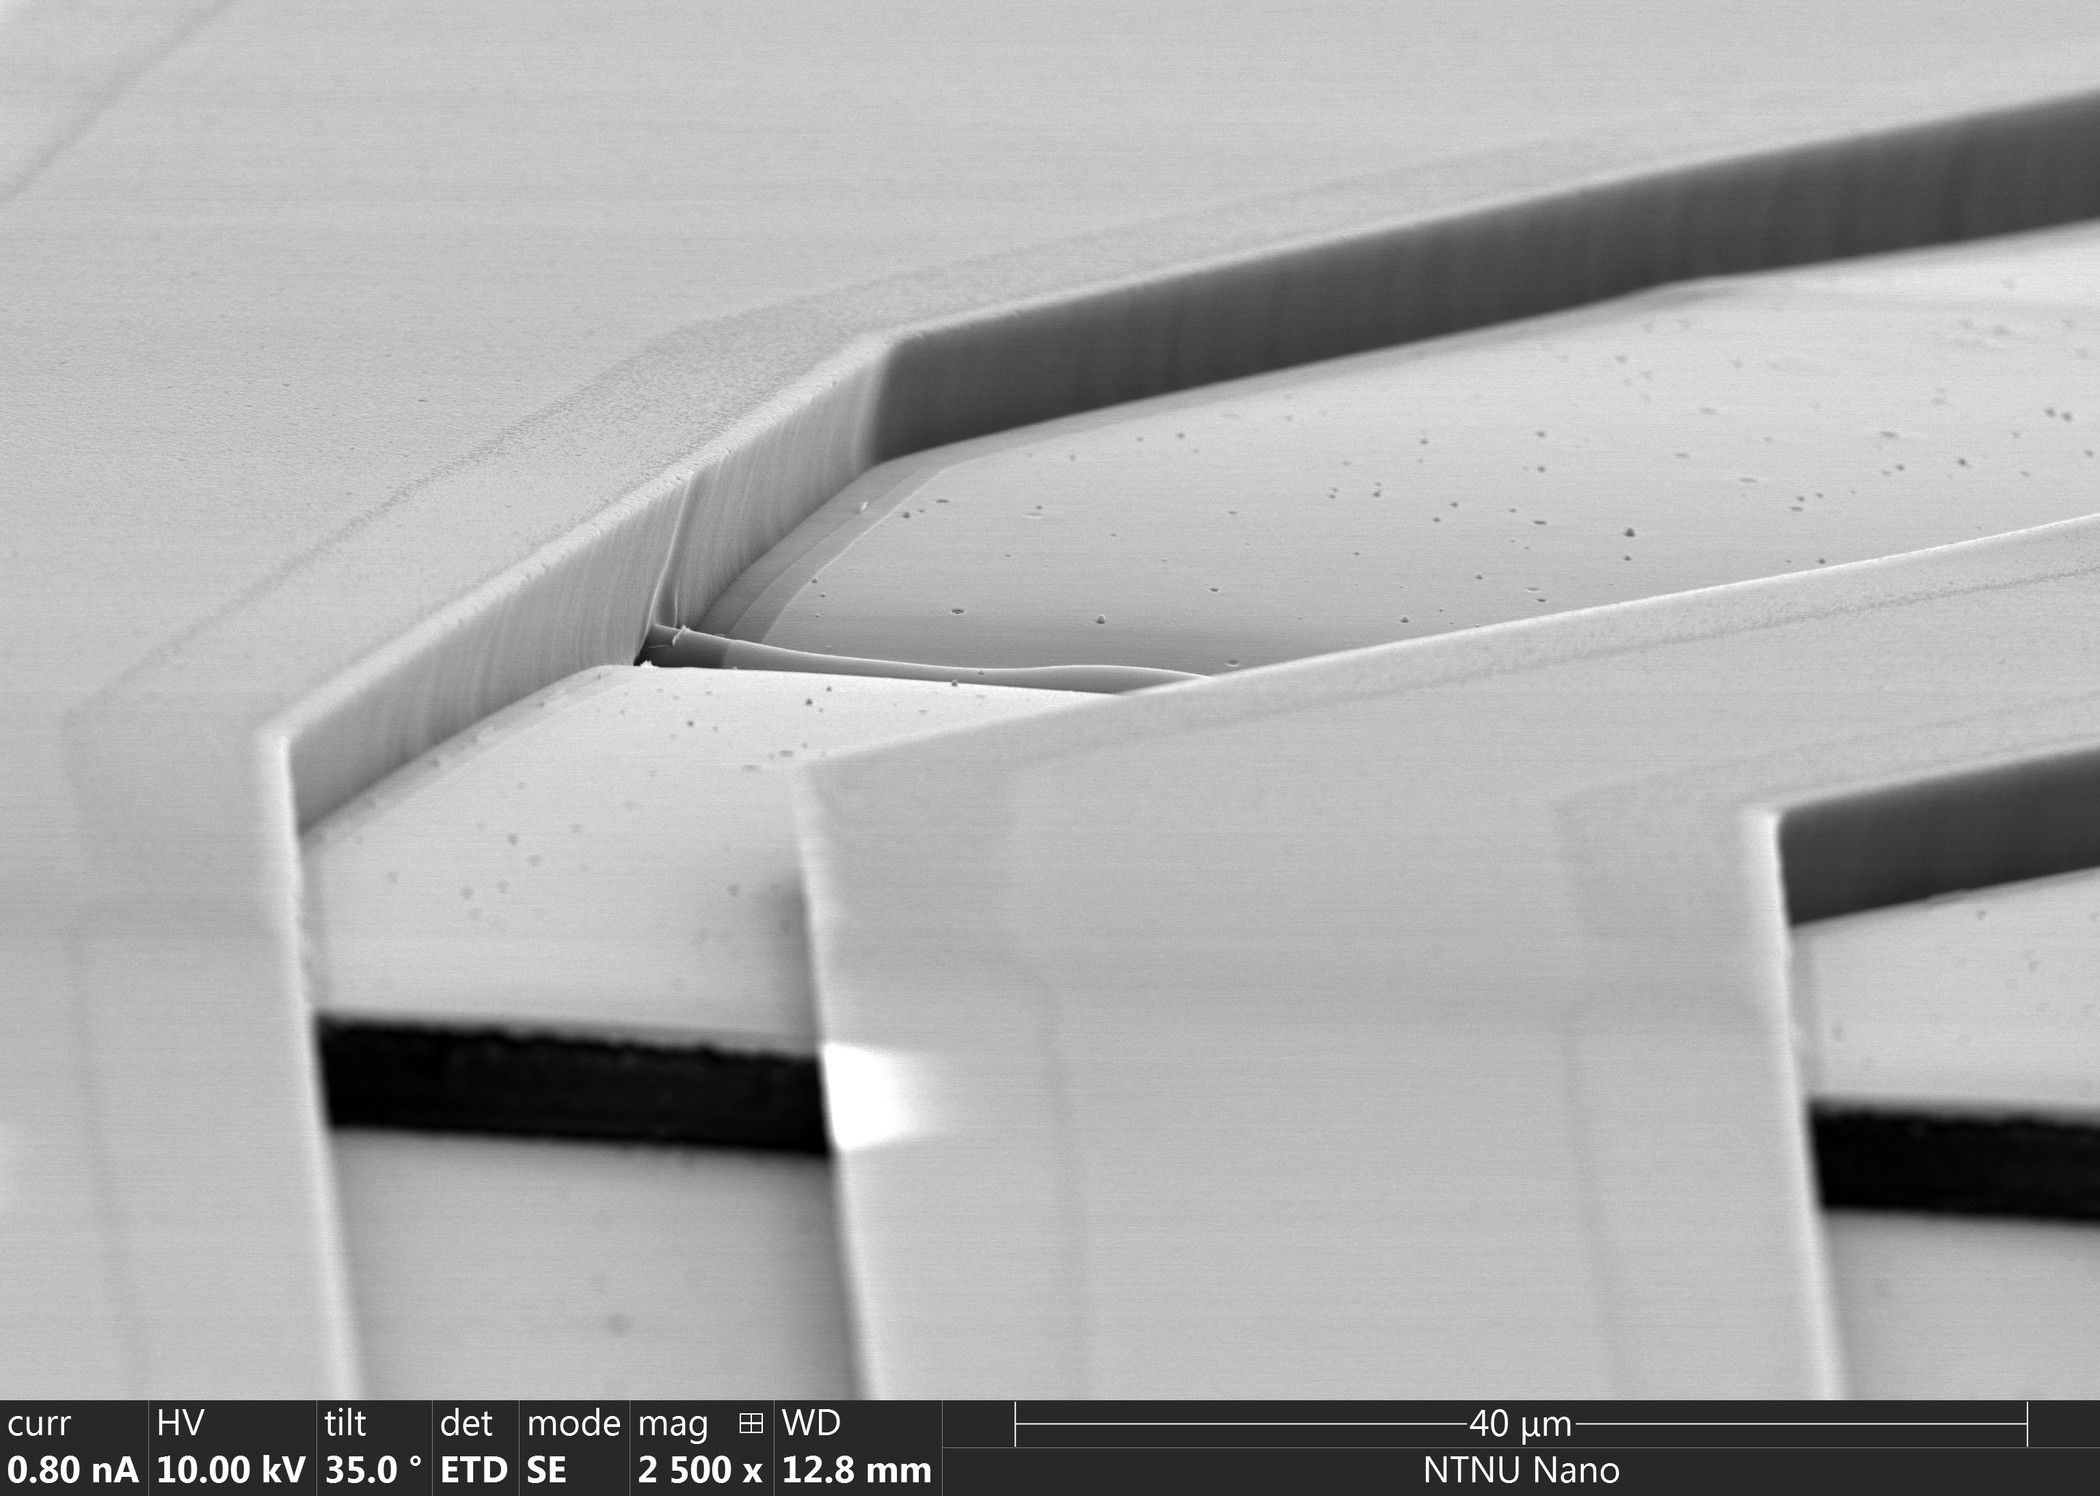
\includegraphics[width=\linewidth]{fig/mr-DWL/mb_25_step_004.jpg}
  %\caption{1a}
 
\end{subfigure}% %blank line makes figures vertical

\caption{}
\label{mrdwl_onfiber}
\end{figure}


\begin{figure}[h!]
 %h here H requires float, exactly here, h! overide latex
\centering
  \centering
  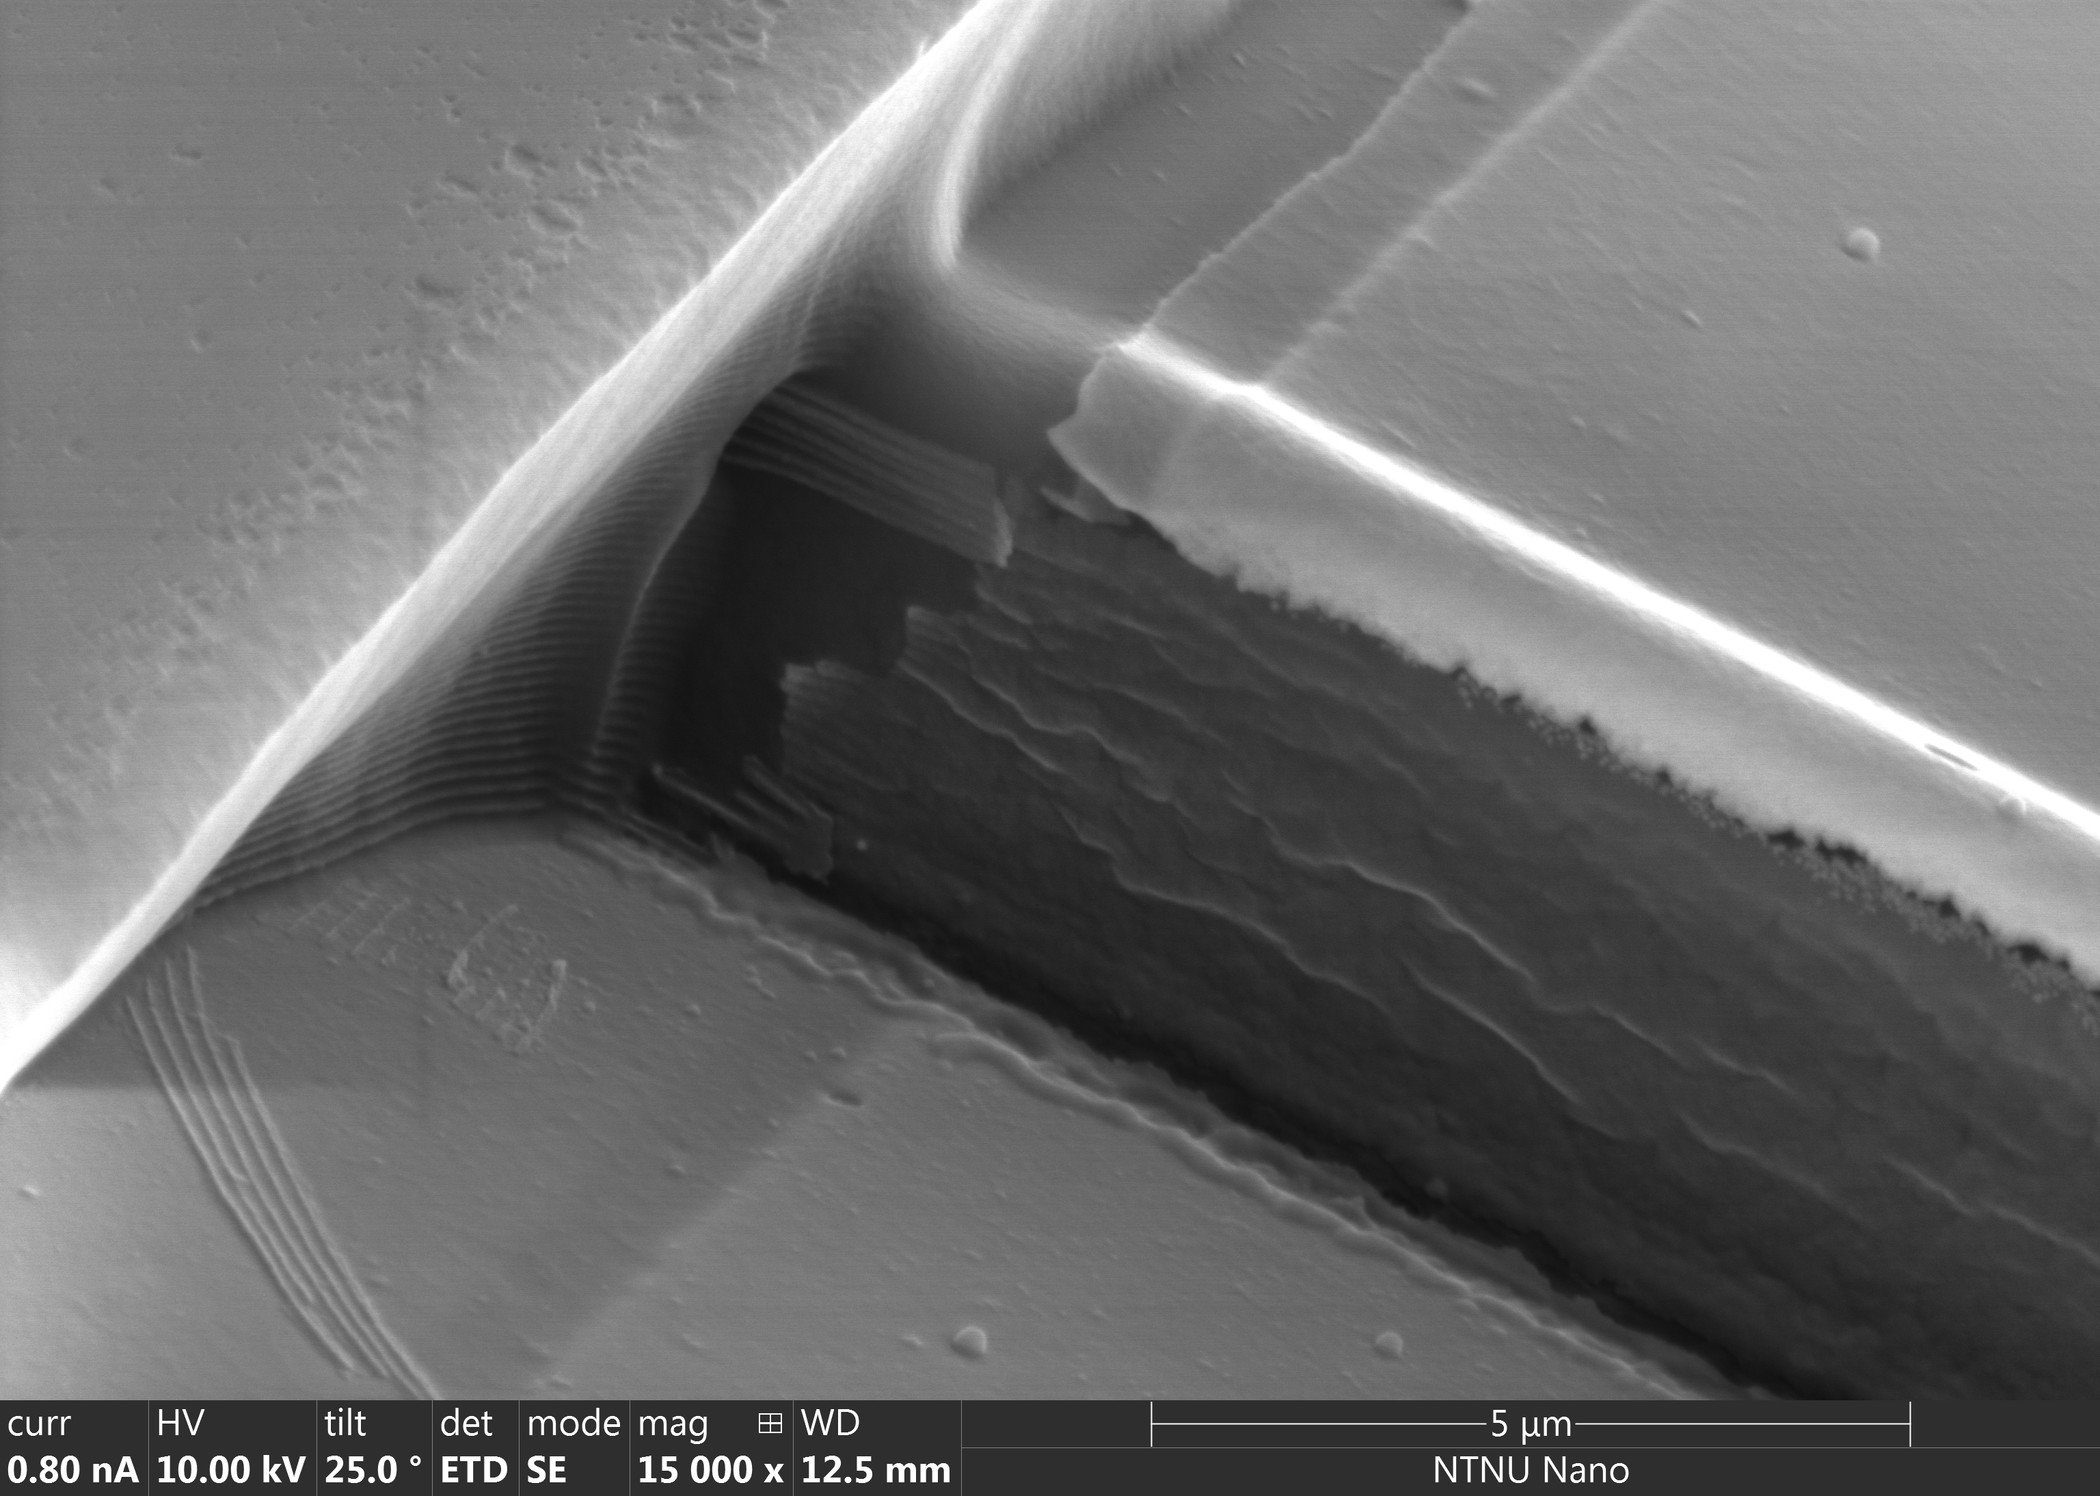
\includegraphics[width=\textwidth]{fig/mr-DWL/mb_25_step_close1.jpg}
  %\caption{1a}
  \label{fig:sfig1}
\caption{}
\label{mrdwl_step}
\end{figure}



\FloatBarrier




\cleardoublepage
